\section{Hiện thực hệ thống}

\subsection{Cấu trúc mã nguồn}
\subsubsection{Ứng dụng web}
    \begin{figure}[H]
    \centering
    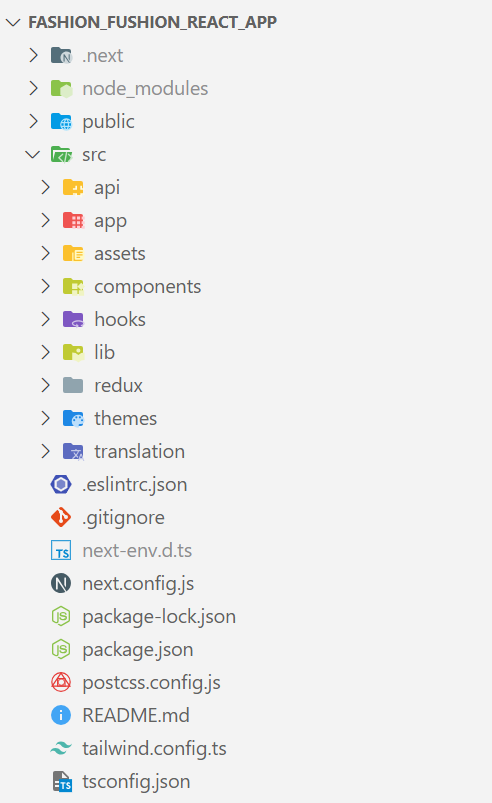
\includegraphics[width=0.6\linewidth]{Images/CodeFolder/WebFolder.png}
    \vspace{20pt}
    \caption{Cấu trúc thư mục ứng dụng web}
    \end{figure}

Tổng quan cấu trúc thư mục chính:
\begin{itemize}
    \item Thư mục api: Giao tiếp giữa Frontend và Backend thông qua api
    \item Thư mục app: Chứa các trang giao diện, layout chính của hệ thống 
    \item Thư mục assets: Chứa các hình ảnh, font chữ, css style sử dụng trong hệ thống
    \item Thư mục components: Chứa các thành phần tái sử dụng của hệ thống
    \item Thư mục hooks: Chứa các custom hooks của React
    \item Thư mục redux: Quản lý các trạng thái toàn cục (global state) của hệ thống
    \item Thư mục themes: Chứa các chủ đề (themes) của hệ thống 
    \item Thư mục translation: Chứa các thư viện, file dịch để sử dụng đa ngôn ngữ cho hệ thống
    
\end{itemize}

\subsubsection{Ứng dụng di động}
\begin{figure}[H]
    \centering
    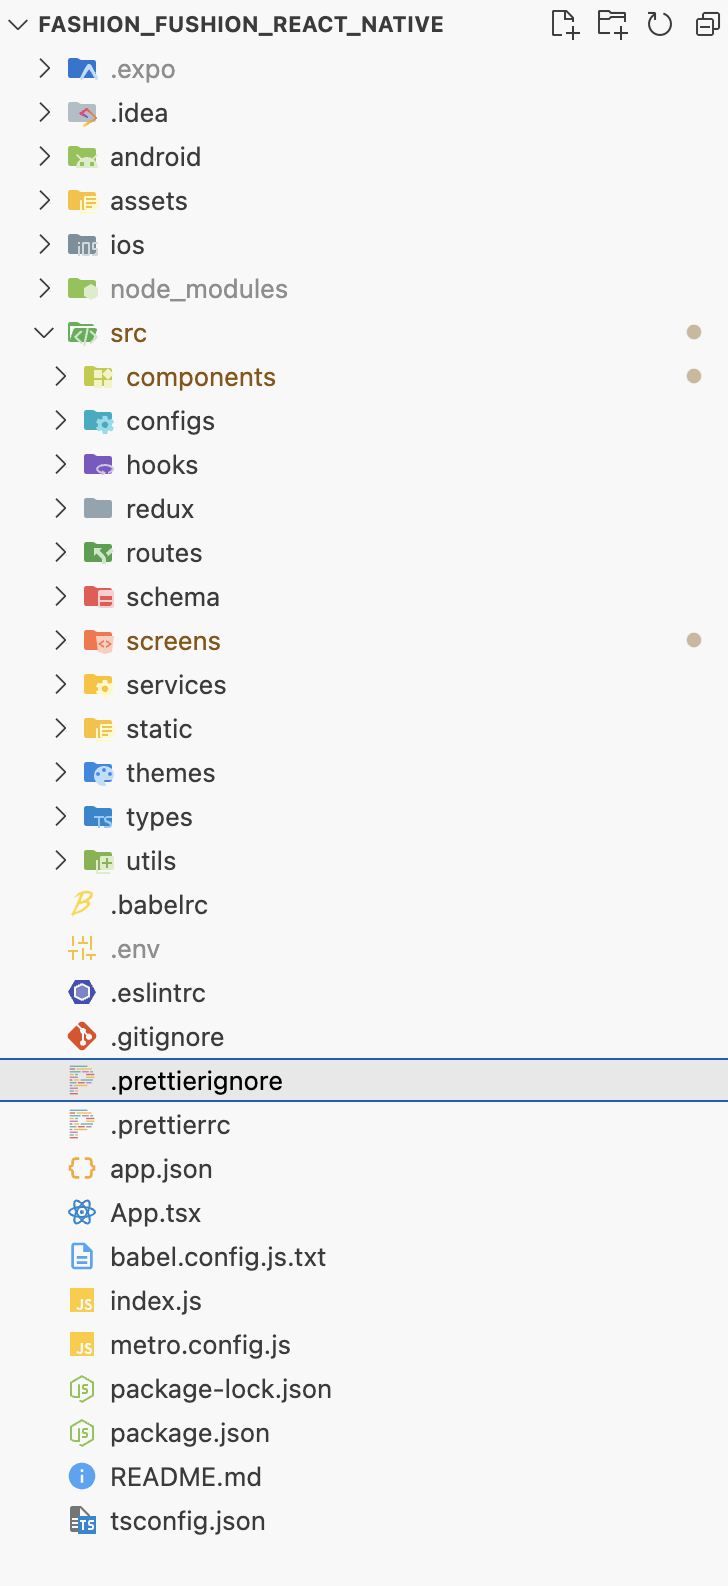
\includegraphics[width=0.4\linewidth]{Images/CodeFolder/mobileFolder.png}
    \vspace{20pt}
    \caption{Cấu trúc thư mục ứng dụng di động}
\end{figure}

Tổng quan cấu trúc thư mục chính:
\begin{itemize}
    \item Thư mục services: Giao tiếp giữa Frontend và Backend thông qua api
    \item Thư mục screens: Chứa tất cả cả màn hình của ứng dụng
    \item Thư mục static: Chứa các hình ảnh, logo và các icon sử dụng
    \item Thư mục components: Chứa các thành phần tái sử dụng của hệ thống
    \item Thư mục redux: Quản lý các trạng thái toàn cục (global state) của hệ thống
    \item Thư mục themes: Chứa các chủ đề (themes) của hệ thống 
    \item Thư mục route: Quản lý điều hướng giữa các màn hình ứng dụng
    \item Thư mục types: dùng để định nghĩa kiểu dữ liệu
    \item Thư mục android và ios: Chứa mã code native
    \item Thư mục util: Chứa các hàm công cụ xử lý
    \item Thư mục config: Chứa các constant và quản lý lỗi
    \item Thư mục hooks: Chứa các hook tự định nghĩa
    \item Thư mục schema: Chứa các cấu trúc dữ liệu và xử lý lỗi trong các Form
\end{itemize}
\subsubsection{Backend}
\begin{figure}[H]
    \centering
    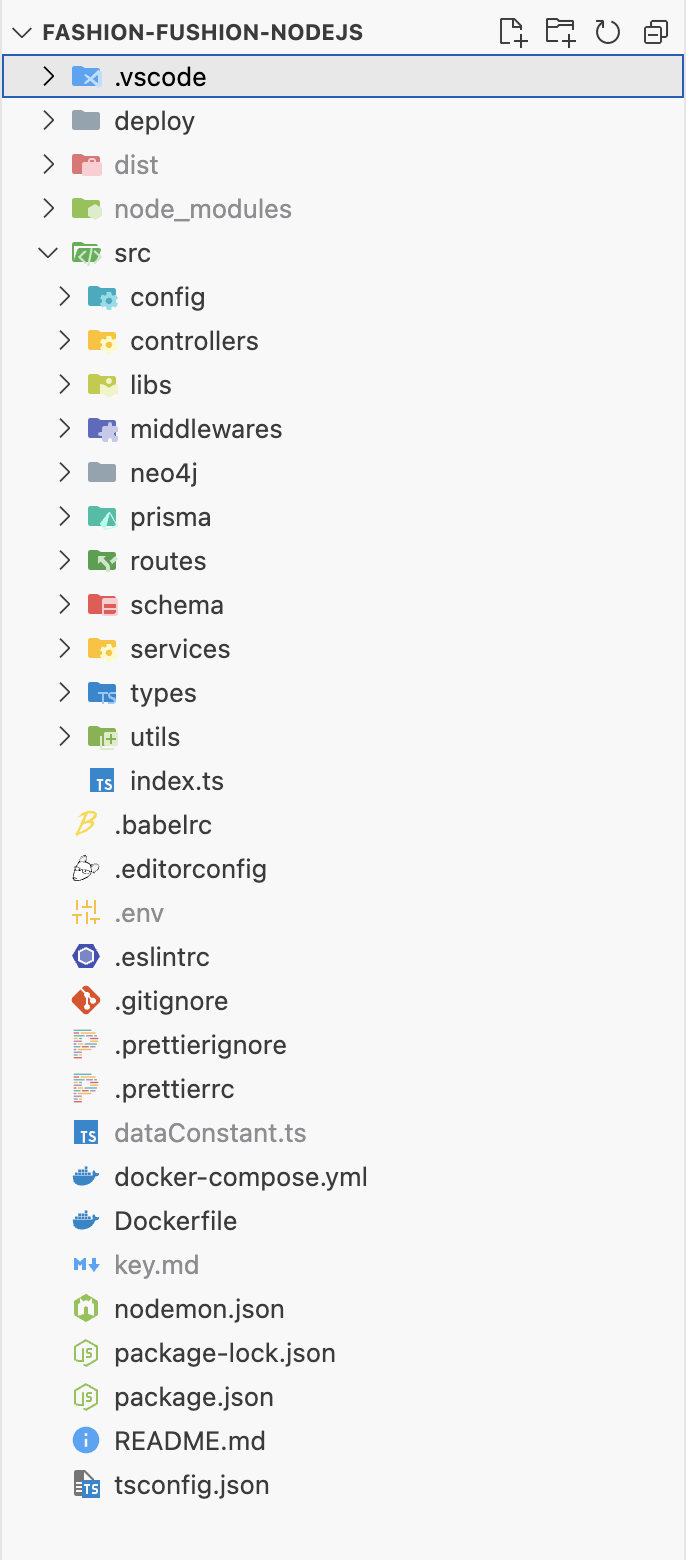
\includegraphics[width=0.4\linewidth]{Images/CodeFolder/backendFolder.png}
    \vspace{20pt}
    \caption{Cấu trúc thư mục Web service}
\end{figure}

Tổng quan cấu trúc thư mục chính:
\begin{itemize}
    \item Thư mục config: Chứa các constant và quản lý lỗi
    \item Thư mục controllers: Chịu trách nhiệm nhận yêu cầu từ client, thực hiện các xử lý cần thiết, và sau đó trả về phản hồi tương ứng
    \item Thư mục libs: Chứa các cài đặt về các thư viện được sử dụng như cổng thanh toán
    \item Thư mục middlewares: Thực hiện các quyền xác thực và xử lý dữ liệu
    \item Thư mục neo4j: Chứa các cài đặt về cơ sở dữ liệu Neo4j
    \item Thư mục prisma: Chứa các cài đặt ORM về cơ sở dữ liệu PosgreSQL
    \item Thư mục routes: Chứa các định nghĩa tuyến đường cho API
    \item Thư mục schema: Chứa các cấu trúc dữ liệu và xử lý lỗi trong các request
    \item Thư mục services: Chứa các thành phần xử lý nghiệp vụ
    \item Thư mục types: dùng để định nghĩa kiểu dữ liệu
    \item Thư mục util: Chứa các hàm công cụ xử lý
\end{itemize}
\subsection{Các API chính}
\begin{table}[H]
\centering
\begin{tabular}{|p{1.5cm}|p{6.5cm}|p{7cm}|}
\hline
Method & URL & Description \\
\hline
POST & /api/order/create & Tạo mới một order  \\
\hline
GET & /api/order/admin & Admin lấy danh sách các order  \\
\hline
GET & /api/order/detail & Lấy thông tin chi tiết của order  \\
\hline
POST & /api/product & Tạo mới một sản phẩm  \\
\hline
POST & /api/product/variant & Tạo mới một variant \\
\hline
POST & /api/product/filter & Filter thông tin và lấy các variant hợp lệ \\
\hline
PATCH & /api/product/variant/image & Thêm ảnh cho variant\\
\hline
GET & /api/product/detail & Lấy thông tin chi tiết của một sản phẩm\\
\hline
GET & /api/user/cart & Lấy các variant từ giỏ hàng\\
\hline
POST & /api/user/cart & Thêm mới một sản phẩm vào giỏ hàng\\
\hline
PATCH & /api/user/cart & Thay đổi số lượng variant trong giỏ hàng\\
\hline
GET & /api/user/wish & Lấy các sản phẩm từ danh sách yêu thích\\
\hline
POST & /api/user/wish & Thêm mới một sản phẩm vào danh sách yêu thích\\
\hline

GET & /api/user/viewed & Lấy các sản phẩm từ danh sách mà người dùng đã xem\\
\hline



\end{tabular}
\end{table}
\newpage

\begin{table}[H]
\centering
\begin{tabular}{|p{1.5cm}|p{6.5cm}|p{7cm}|}
\hline
Method & URL & Description \\
\hline
POST & /api/user/viewed & Thêm mới một sản phẩm vào danh sách mà người dùng đã xem\\
\hline
GET & /api/user/recommendbyuser & Lấy các sản phẩm được gợi ý cho người dùng\\
\hline
POST & /api/user/recommendbyotheruser & Lấy các sản phẩm được gợi ý từ người dùng khác\\
\hline
POST & /api/review & Tạo mới một review\\
\hline
PATCH & /api/review/is-disable & Staff cập nhật disable cho review\\
\hline
GET & /api/staff/over-view & Staff lấy các thông tin overview của trang dashboard\\
\hline
GET & /api/staff/revenue & Staff lấy các thông tin doanh thu theo từng ngày trong khoảng thời gian chỉ định\\
\hline
GET & /api/staff/best-selling & Staff lấy các thông tin các sản phẩm có số lượng mua cao nhất trong khoảng thời gian chỉ định\\
\hline
POST & /fastapi/upload & Chuyển ảnh của các sản phẩm thành các vector\\
\hline
POST & /fastapi/search\_base64 & Nhận ảnh của người dùng để tiến hành tìm kiếm ảnh tương đồng\\
\hline
POST & /api/voucher & Tạo mới một voucher\\
\hline

\end{tabular}
\caption{Bảng các API chính}
\end{table}

\subsection{Giao diện hệ thống}
\subsubsection{Giao diện web của quản trị viên}

\begin{itemize}
    \item \textbf{Trang điều khiển (Dashboard)}
\end{itemize}
 \begin{figure}[H]
        \centering
        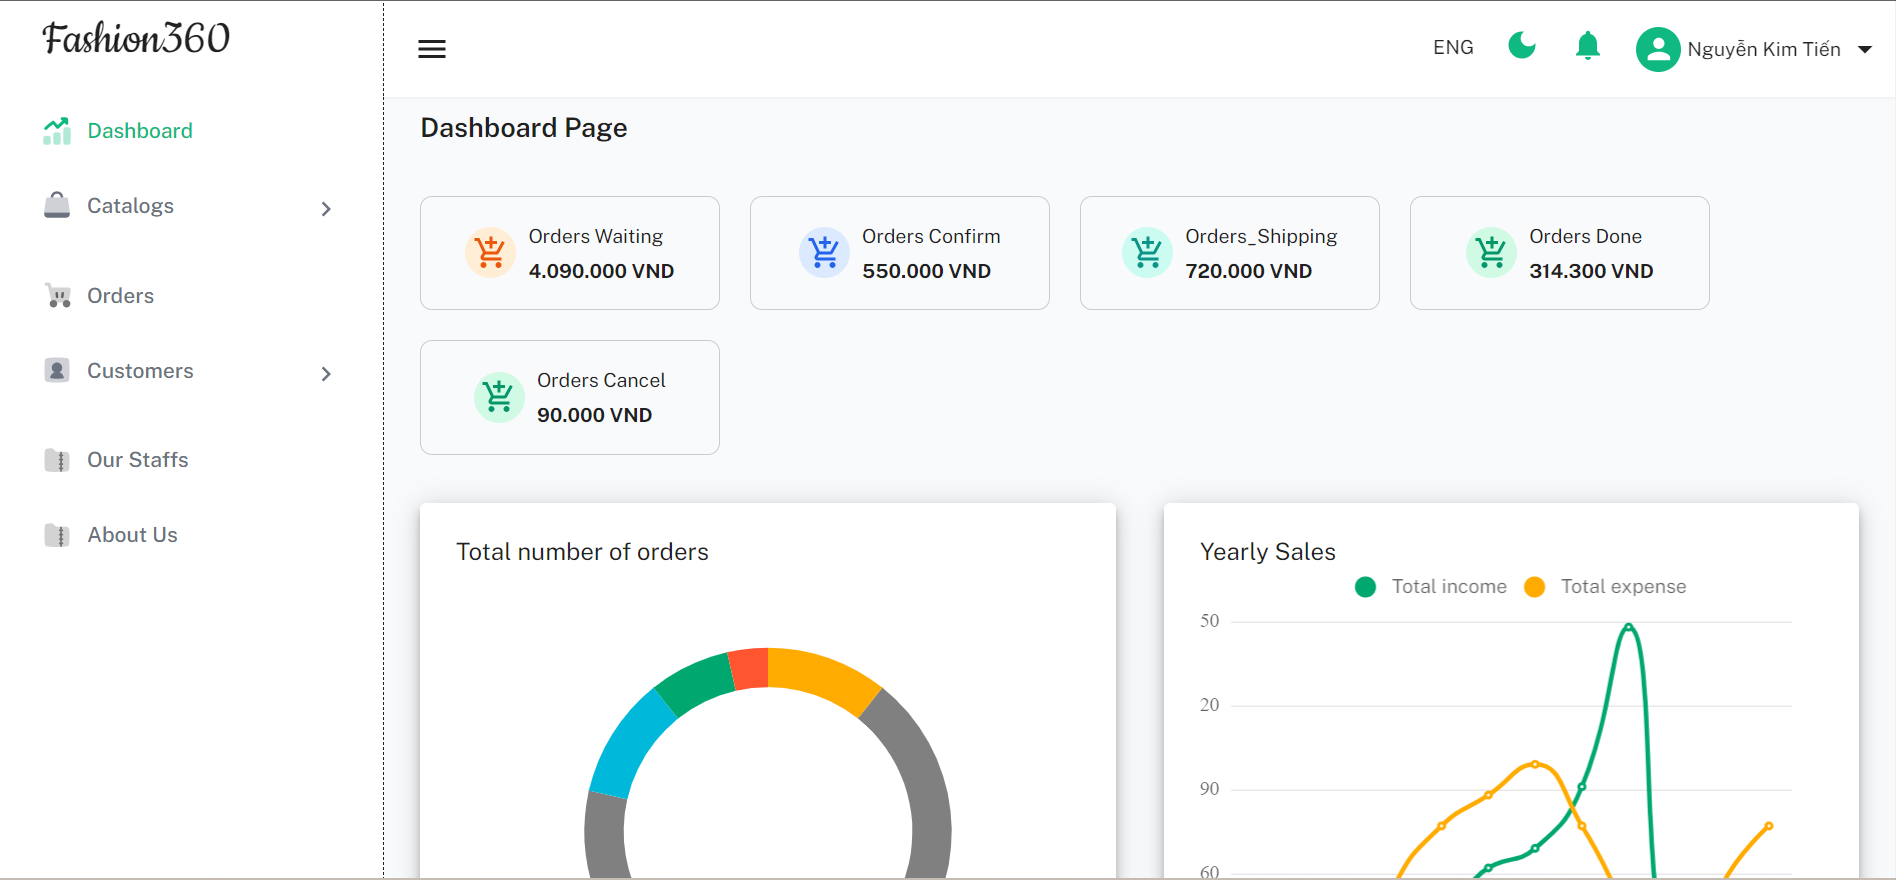
\includegraphics[width=14cm]{Images/Web/dashboard.png}
        \newline
        \caption{Một phần giao diện của trang điều khiển (Dashboard)}
\end{figure}
 \begin{figure}[H]
        \centering
        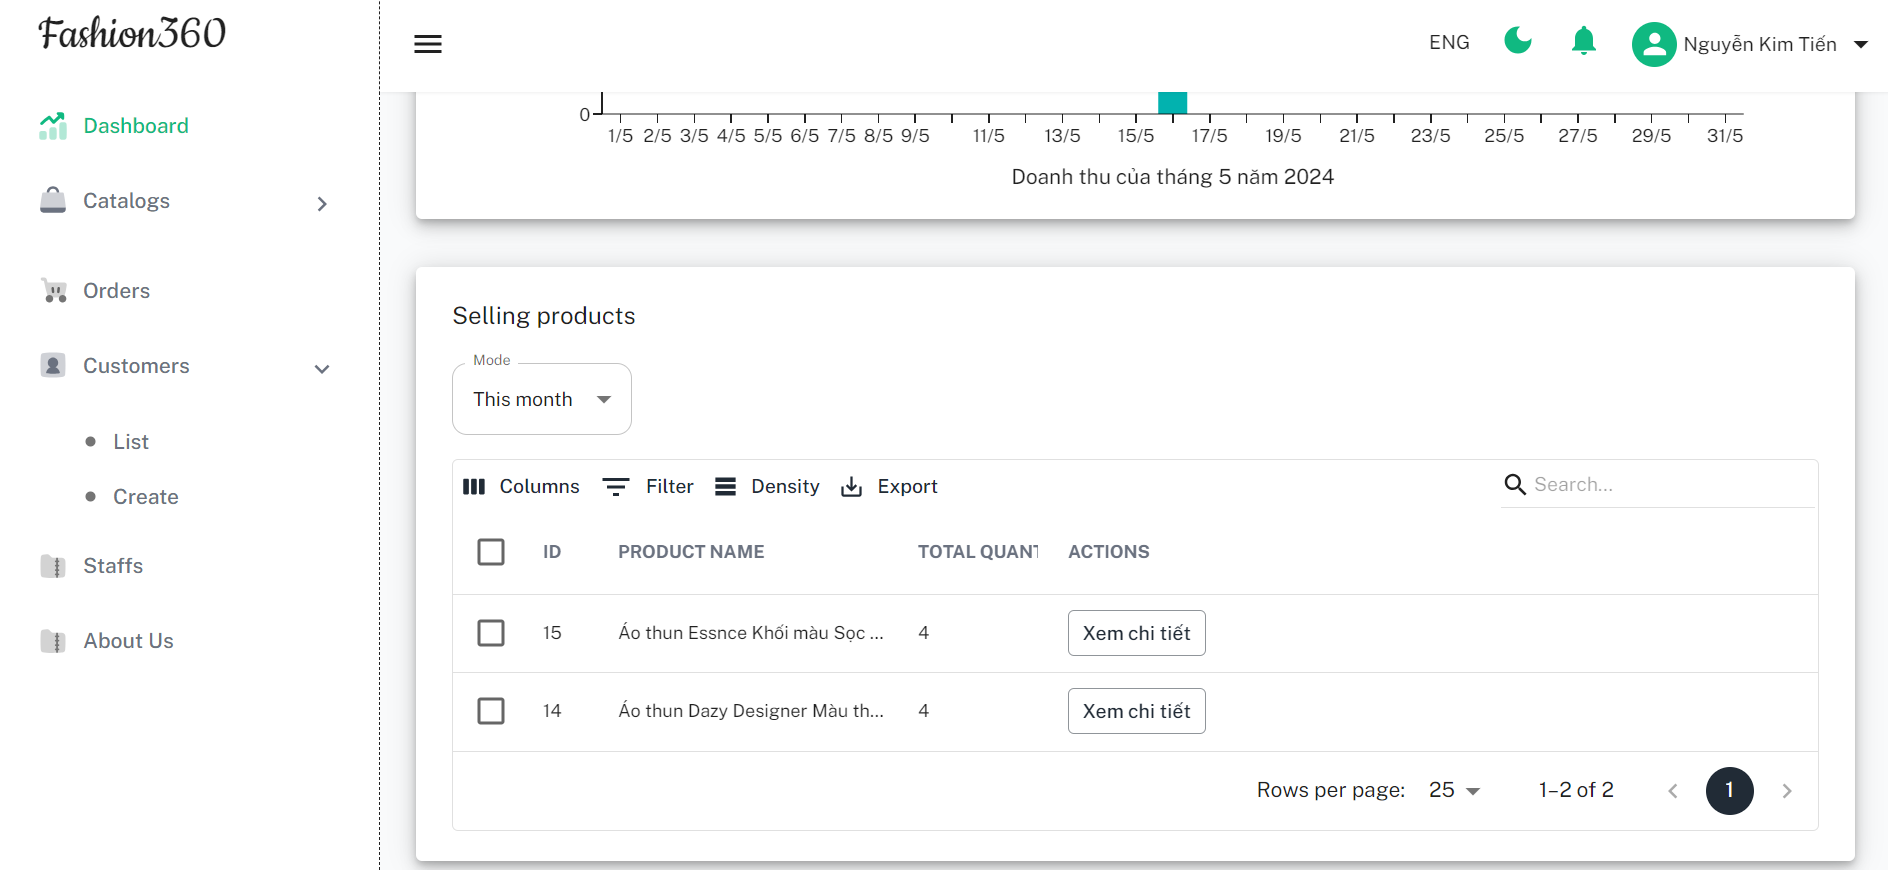
\includegraphics[width=14cm]{Images/Web/dashboard2.png}
        \newline
        \caption{Một phần giao diện của trang điều khiển (Dashboard)}
\end{figure}

\begin{itemize}
    \item \textbf{Trang thể loại (Category)}
\end{itemize}
 \begin{figure}[H]
        \centering
        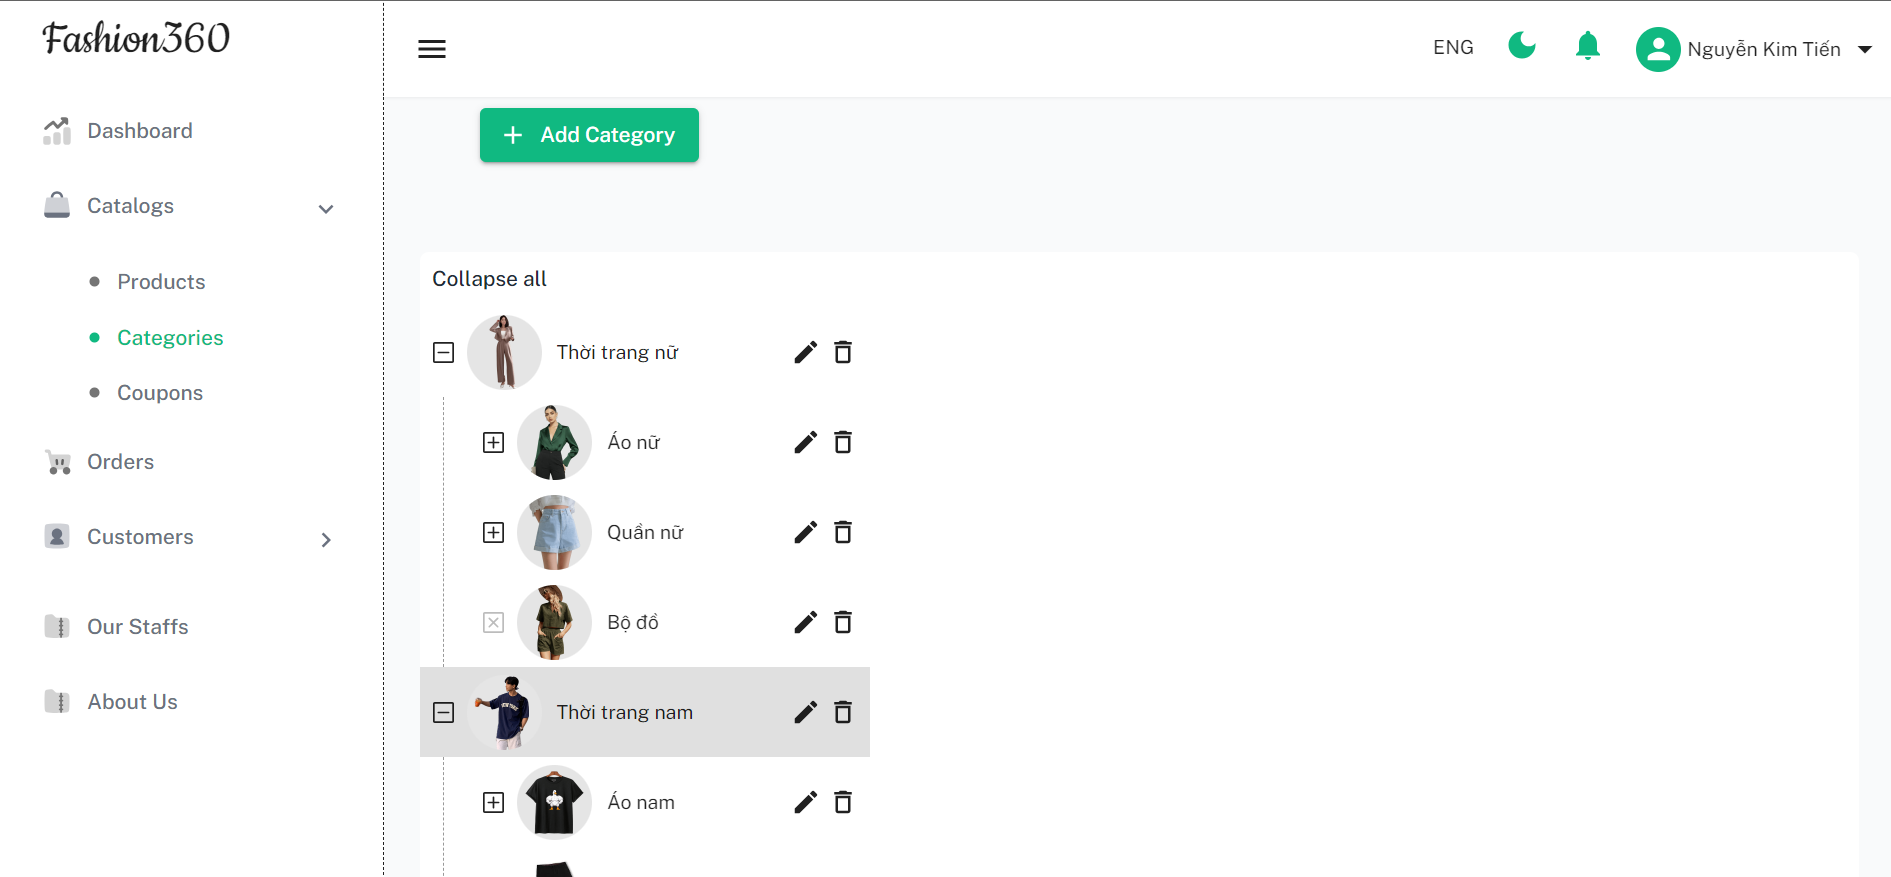
\includegraphics[width=14cm]{Images/Web/category.png}
        \newline
        \caption{Giao diện hiển thị danh sách thể loại}
\end{figure}
\begin{figure}[H]
        \centering
        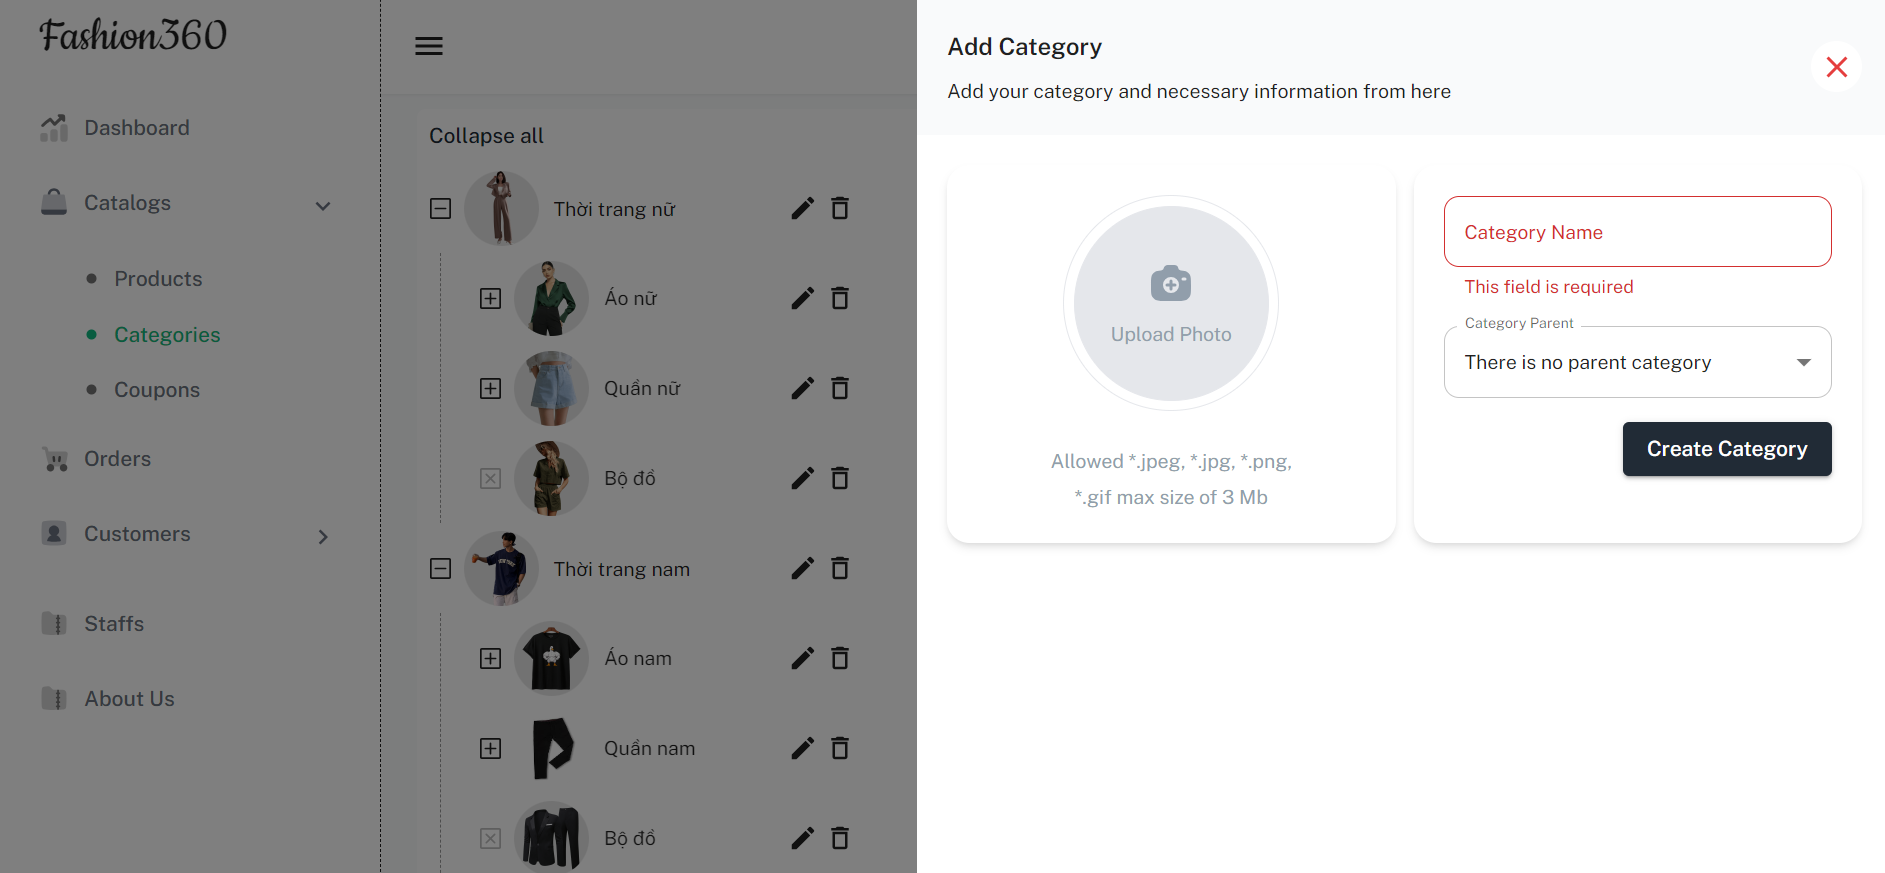
\includegraphics[width=14cm]{Images/Web/addCategory.png}
        \newline
        \caption{Giao diện của trang tạo mới thể loại}
\end{figure}
\begin{figure}[H]
        \centering
        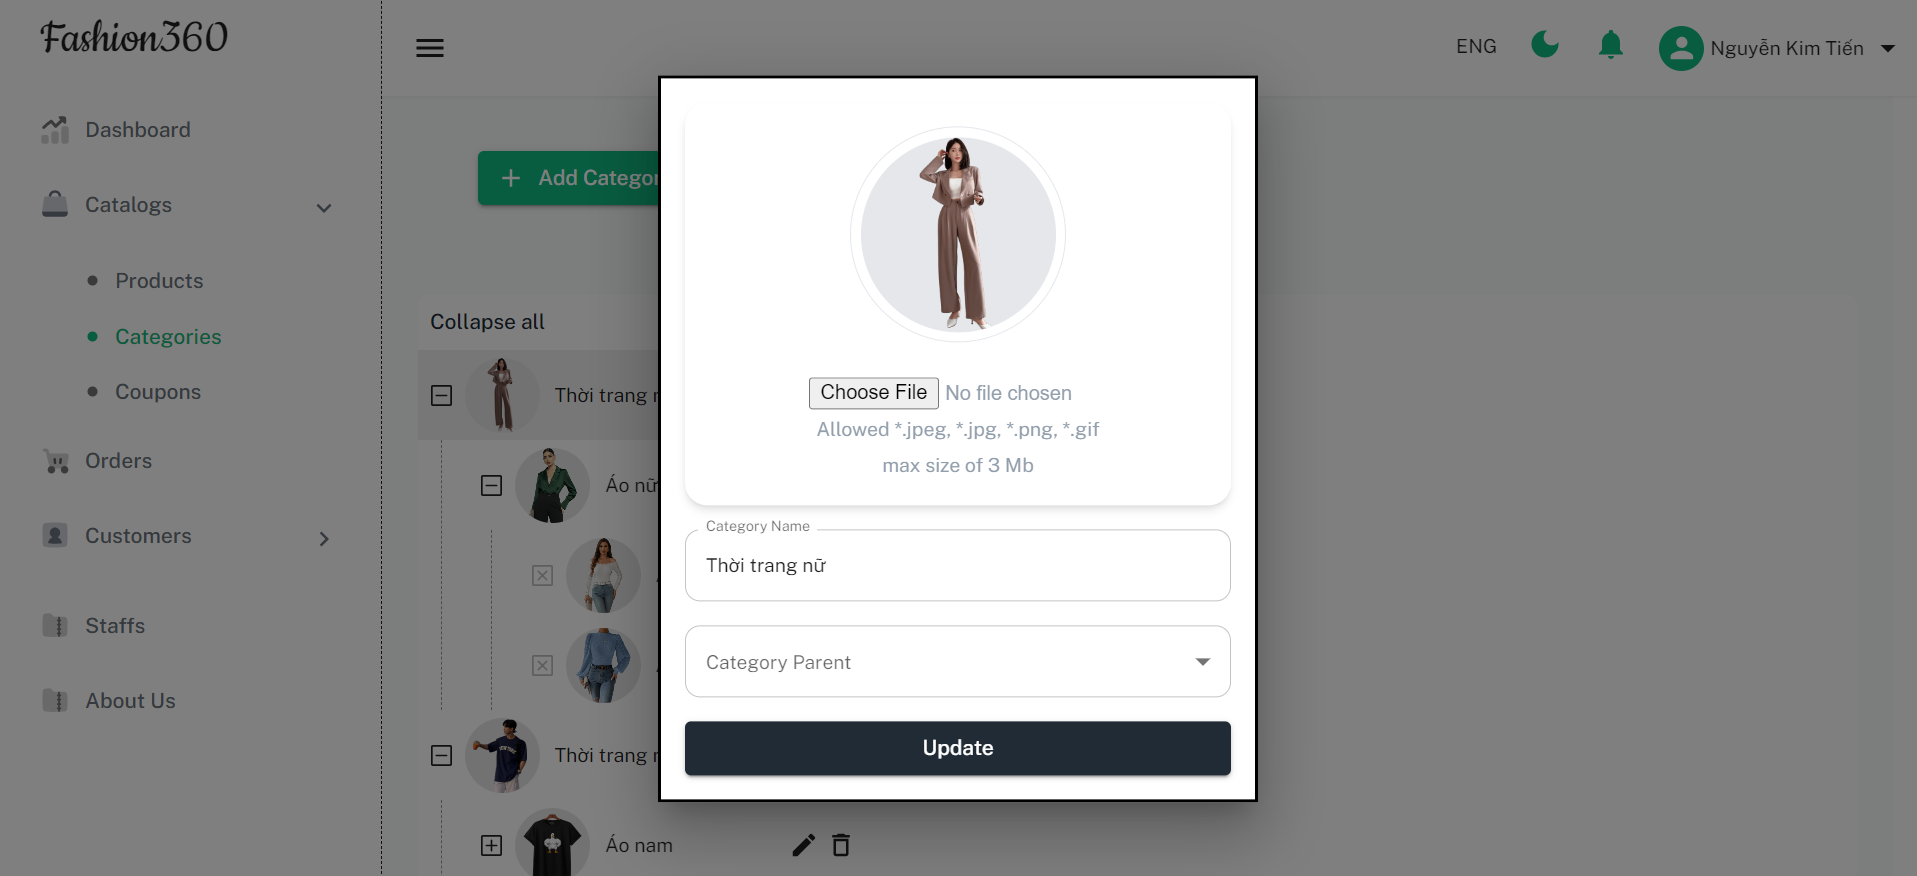
\includegraphics[width=14cm]{Images/Web/updateCategory.png}
        \newline
        \caption{Giao diện của trang cập nhật thể loại}
\end{figure}

\begin{itemize}
    \item \textbf{Trang sản phẩm (Product)}
\end{itemize}
 \begin{figure}[H]
        \centering
        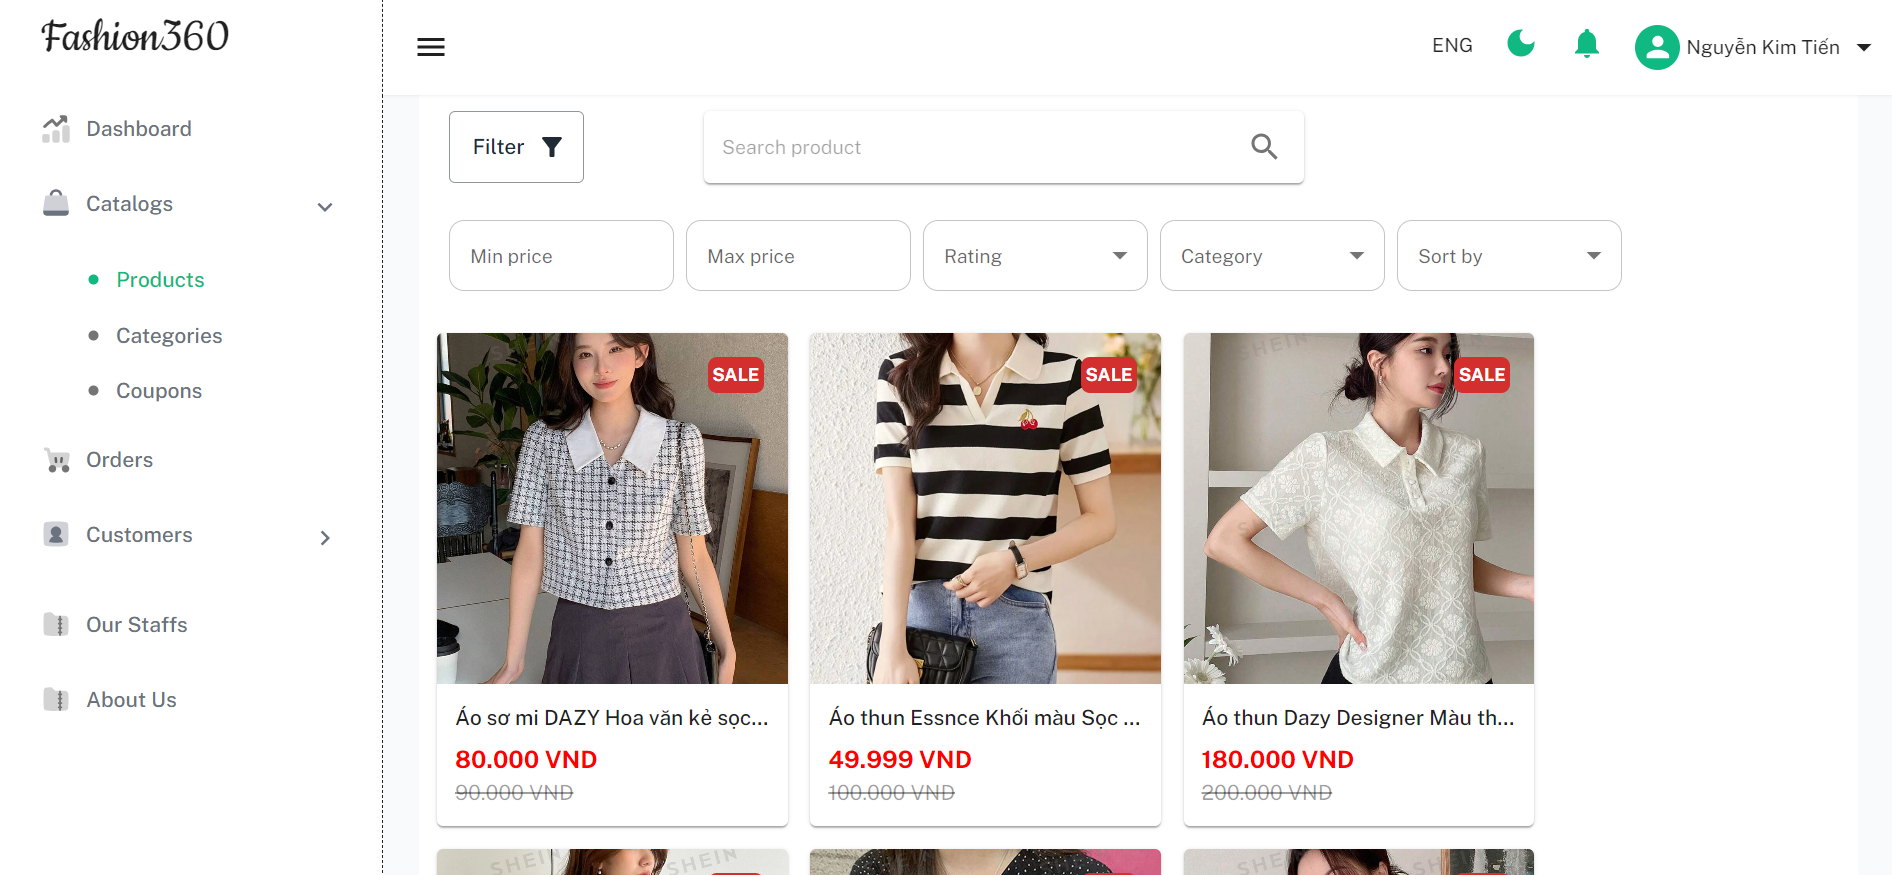
\includegraphics[width=14cm]{Images/Web/productList.png}
        \newline
        \caption{Một phần giao diện hiển thị danh sách sản phẩm}
\end{figure}
 \begin{figure}[H]
        \centering
        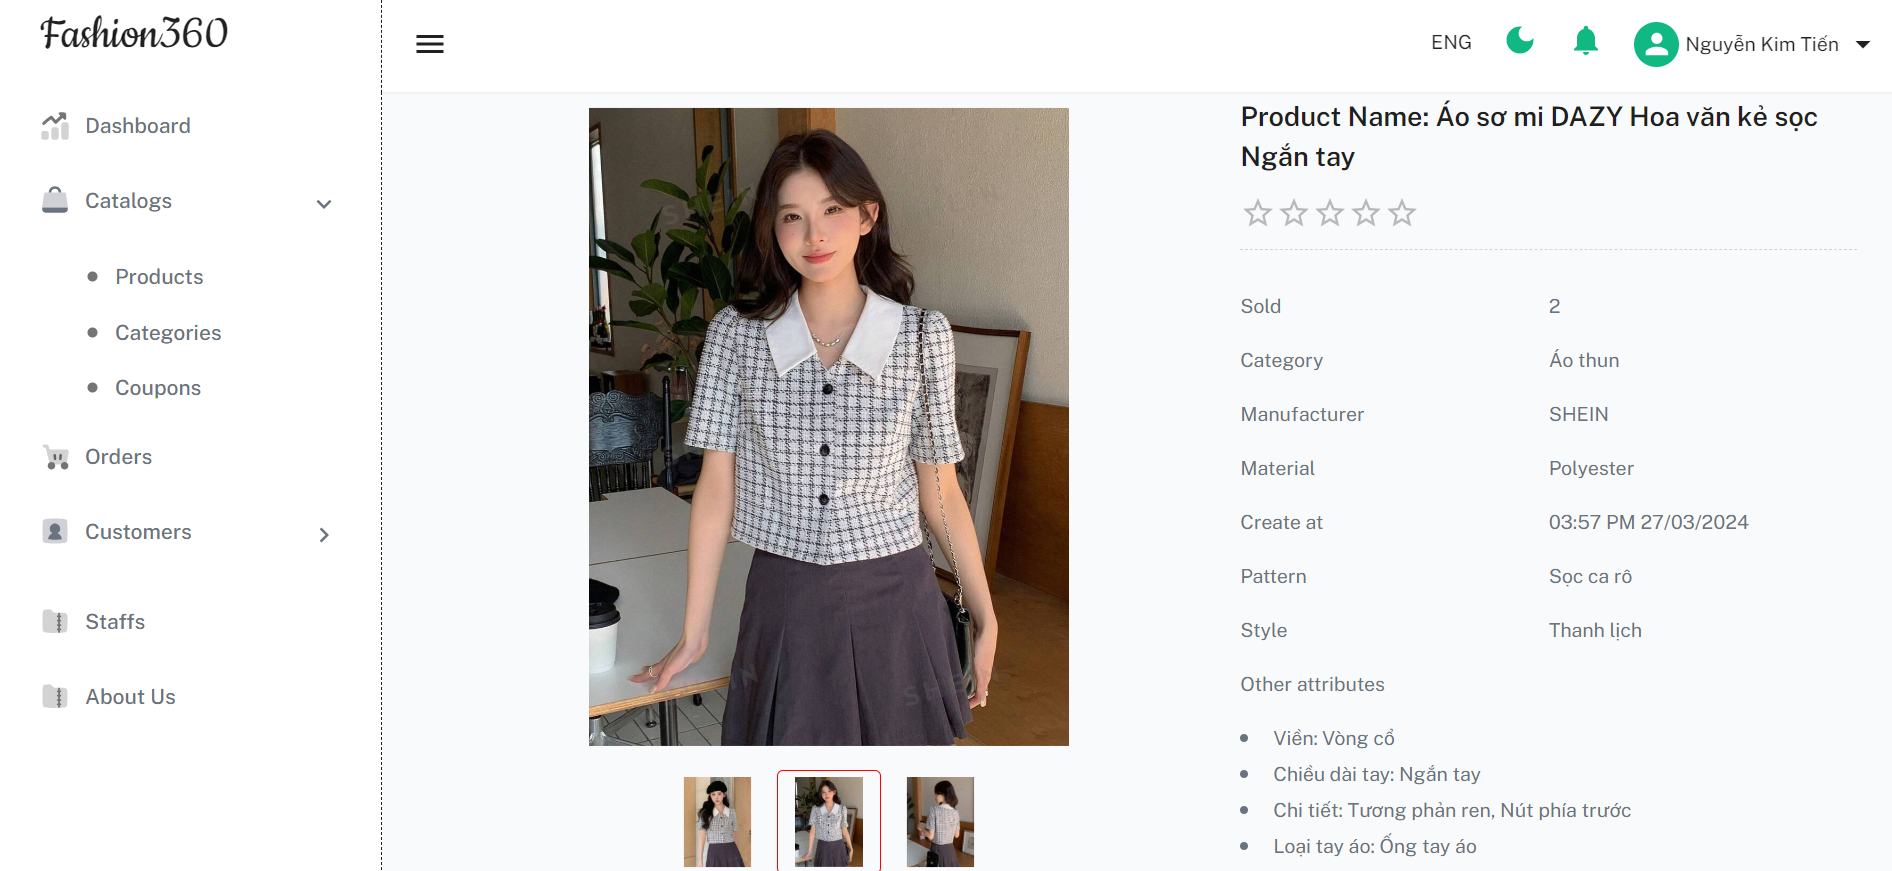
\includegraphics[width=14cm]{Images/Web/productDetail.png}
        \newline
        \caption{Một phần giao diện hiển thị thông tin chi tiết sản phẩm}
\end{figure}
\begin{figure}[H]
        \centering
        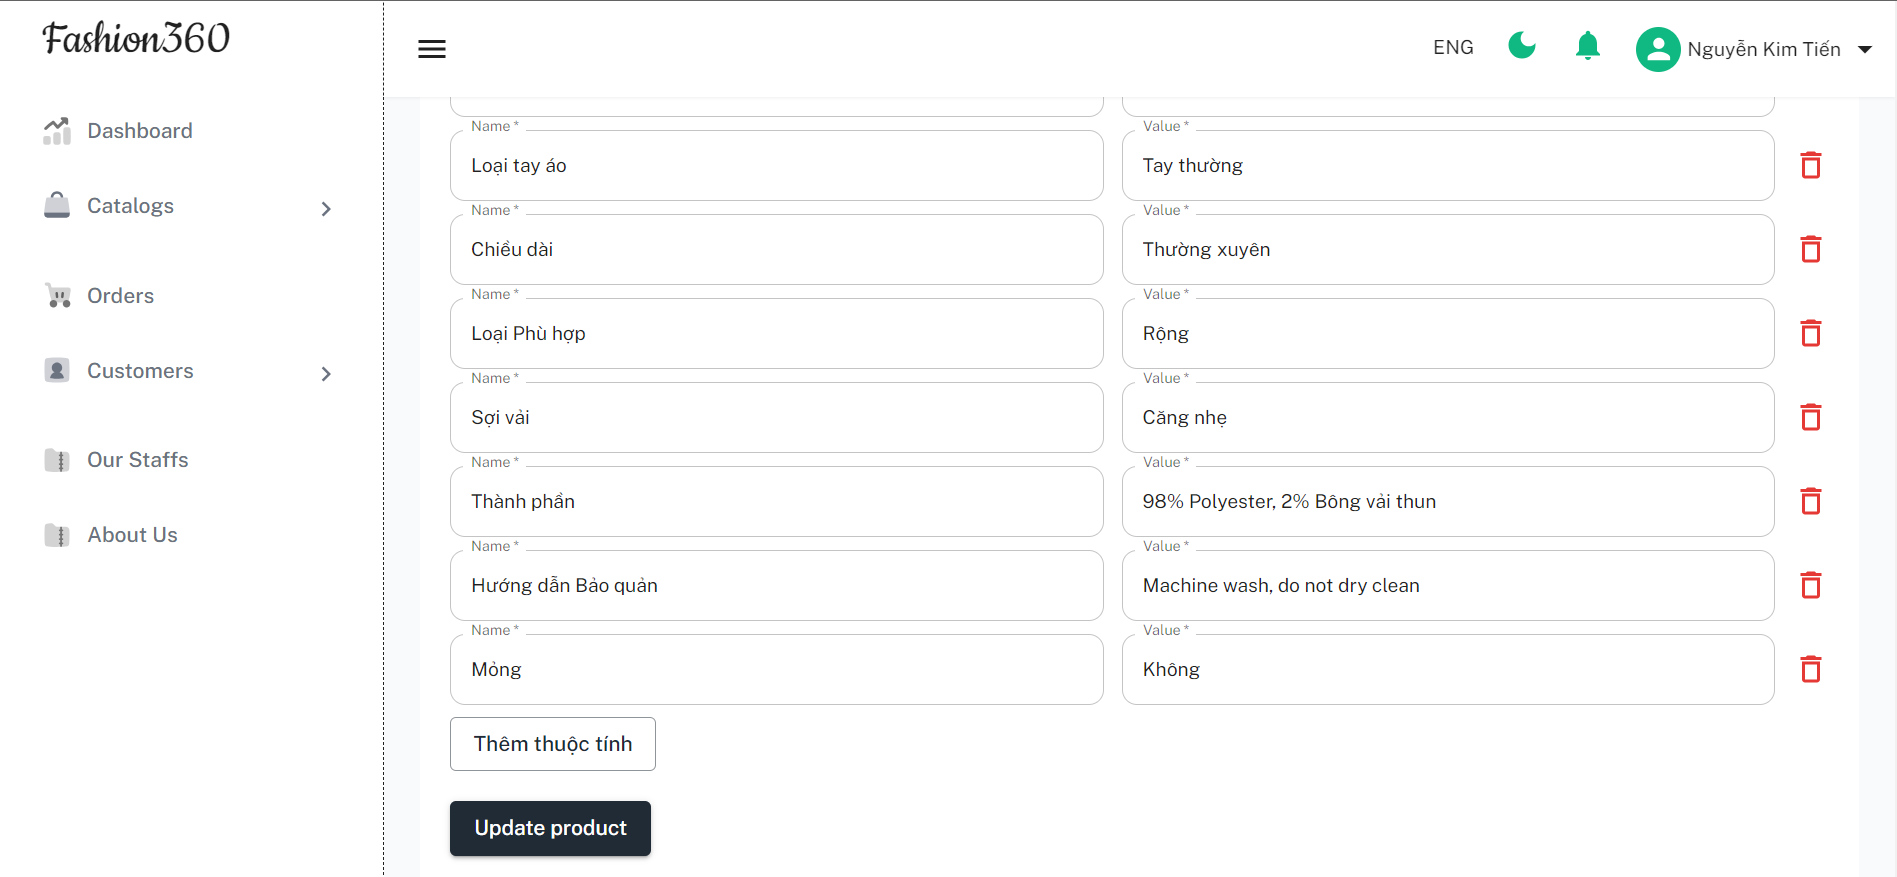
\includegraphics[width=14cm]{Images/Web/updateProduct.png}
        \newline
        \caption{Một phần giao diện của trang cập nhật sản phẩm}
\end{figure}

\begin{itemize}
    \item \textbf{Trang Variant}
\end{itemize}
 \begin{figure}[H]
        \centering
        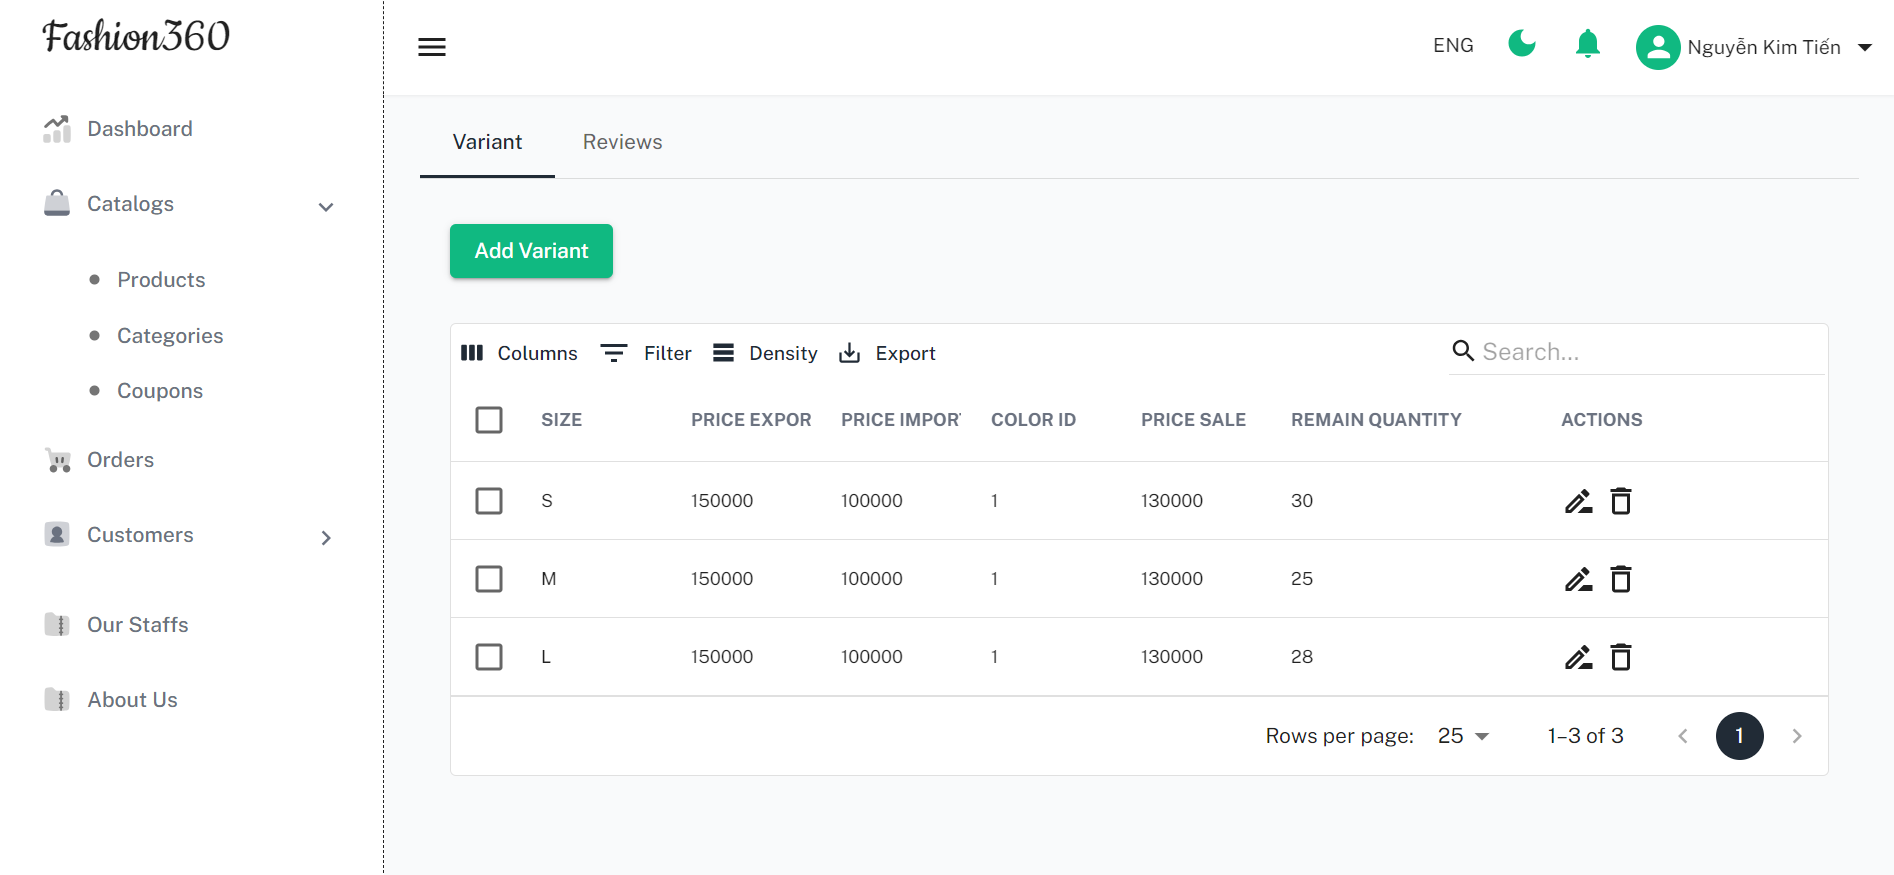
\includegraphics[width=14cm]{Images/Web/variant.png}
        \newline
        \caption{Một phần giao diện hiển thị danh sách Variant}
\end{figure}
 \begin{figure}[H]
        \centering
        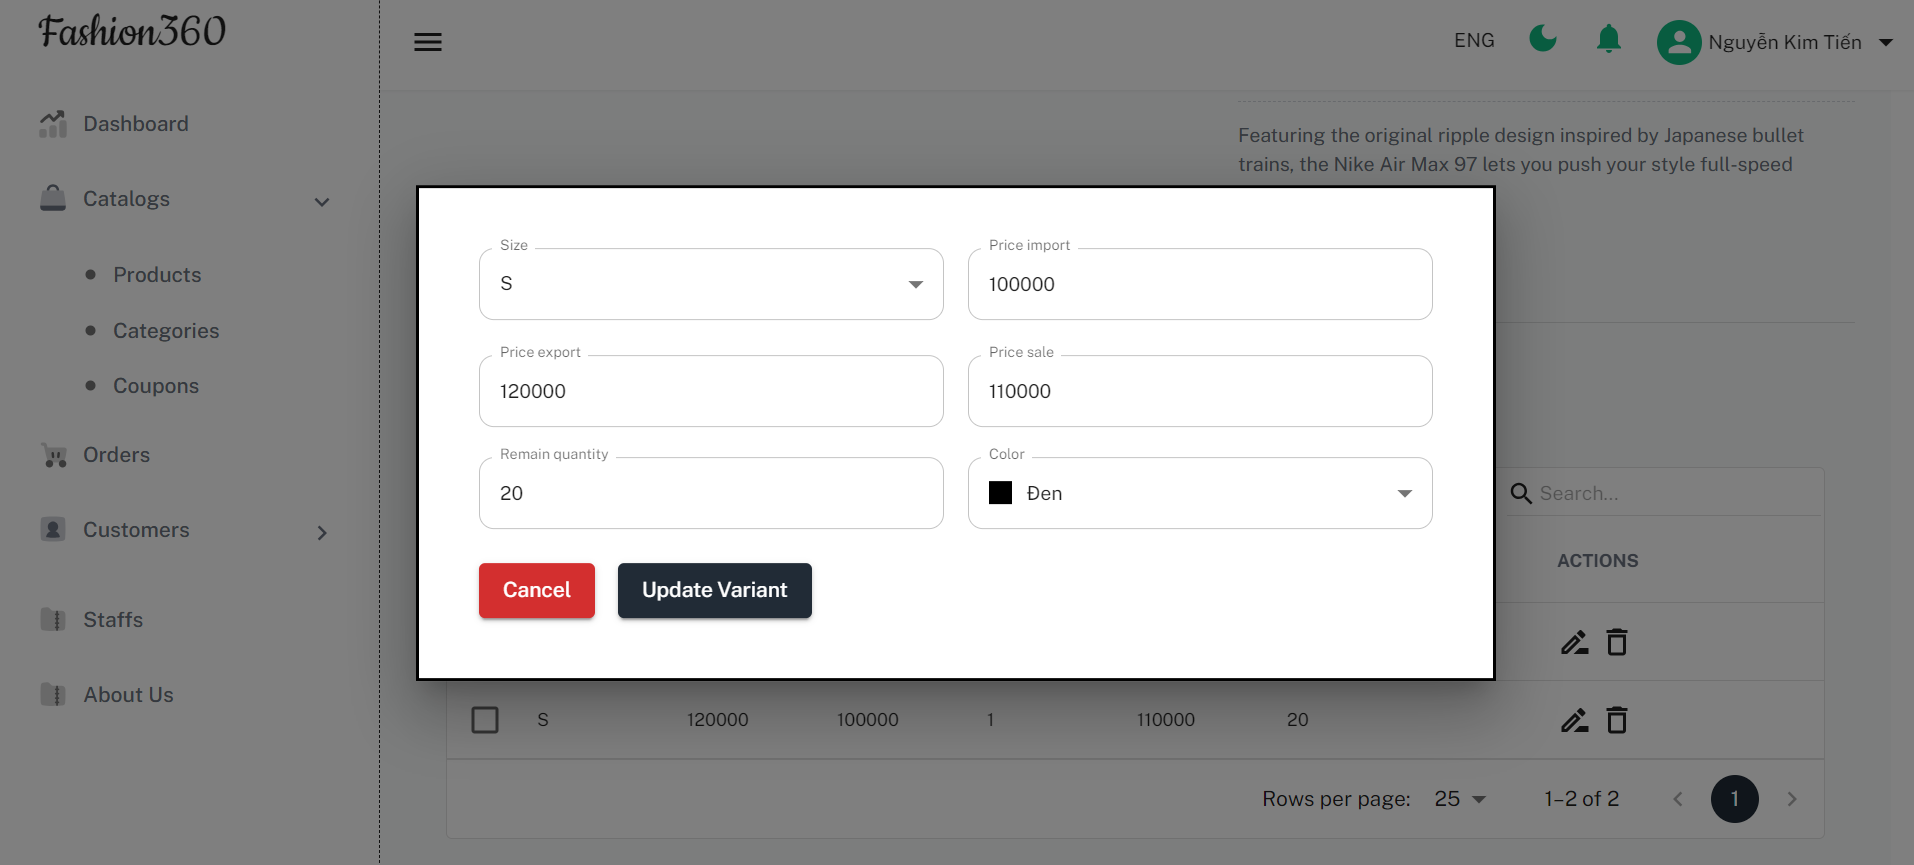
\includegraphics[width=14cm]{Images/Web/updateVariant.png}
        \newline
        \caption{Giao diện của trang cập nhật Variant}
\end{figure}

\begin{itemize}
    \item \textbf{Trang mã giảm giá (Coupons)}
\end{itemize}
 \begin{figure}[H]
        \centering
        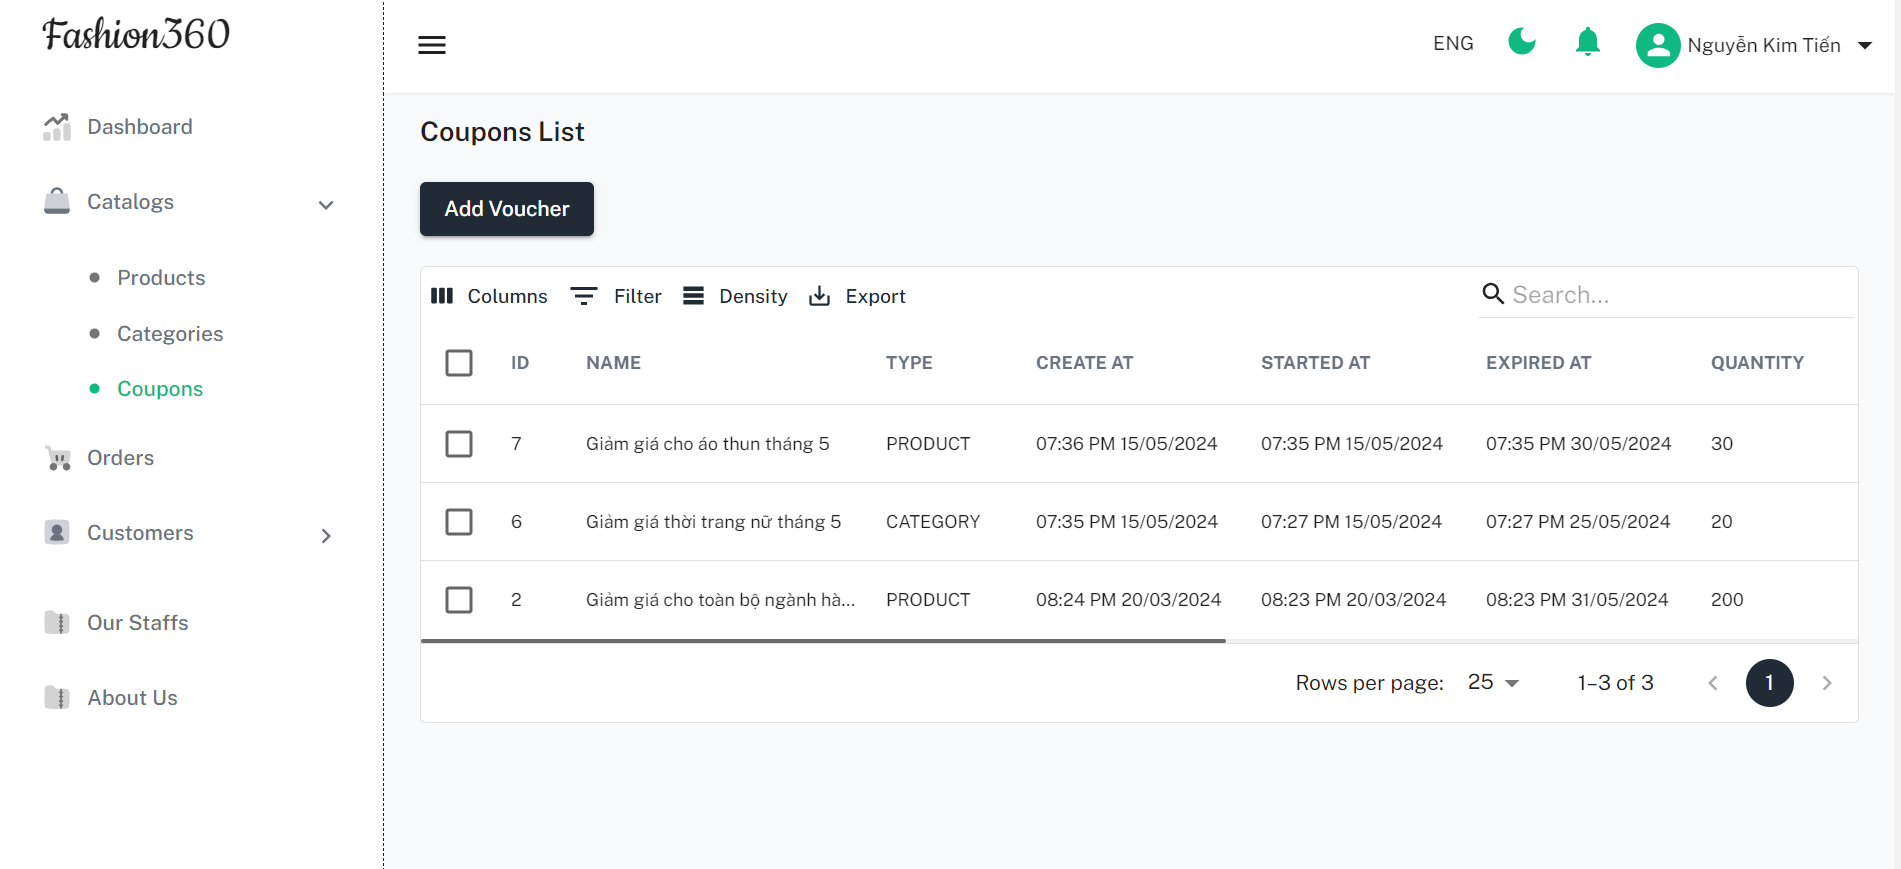
\includegraphics[width=14cm]{Images/Web/voucher.png}
        \newline
        \caption{Giao diện hiển thị danh sách mã giảm giá}
\end{figure}

\begin{figure}[H]
        \centering
        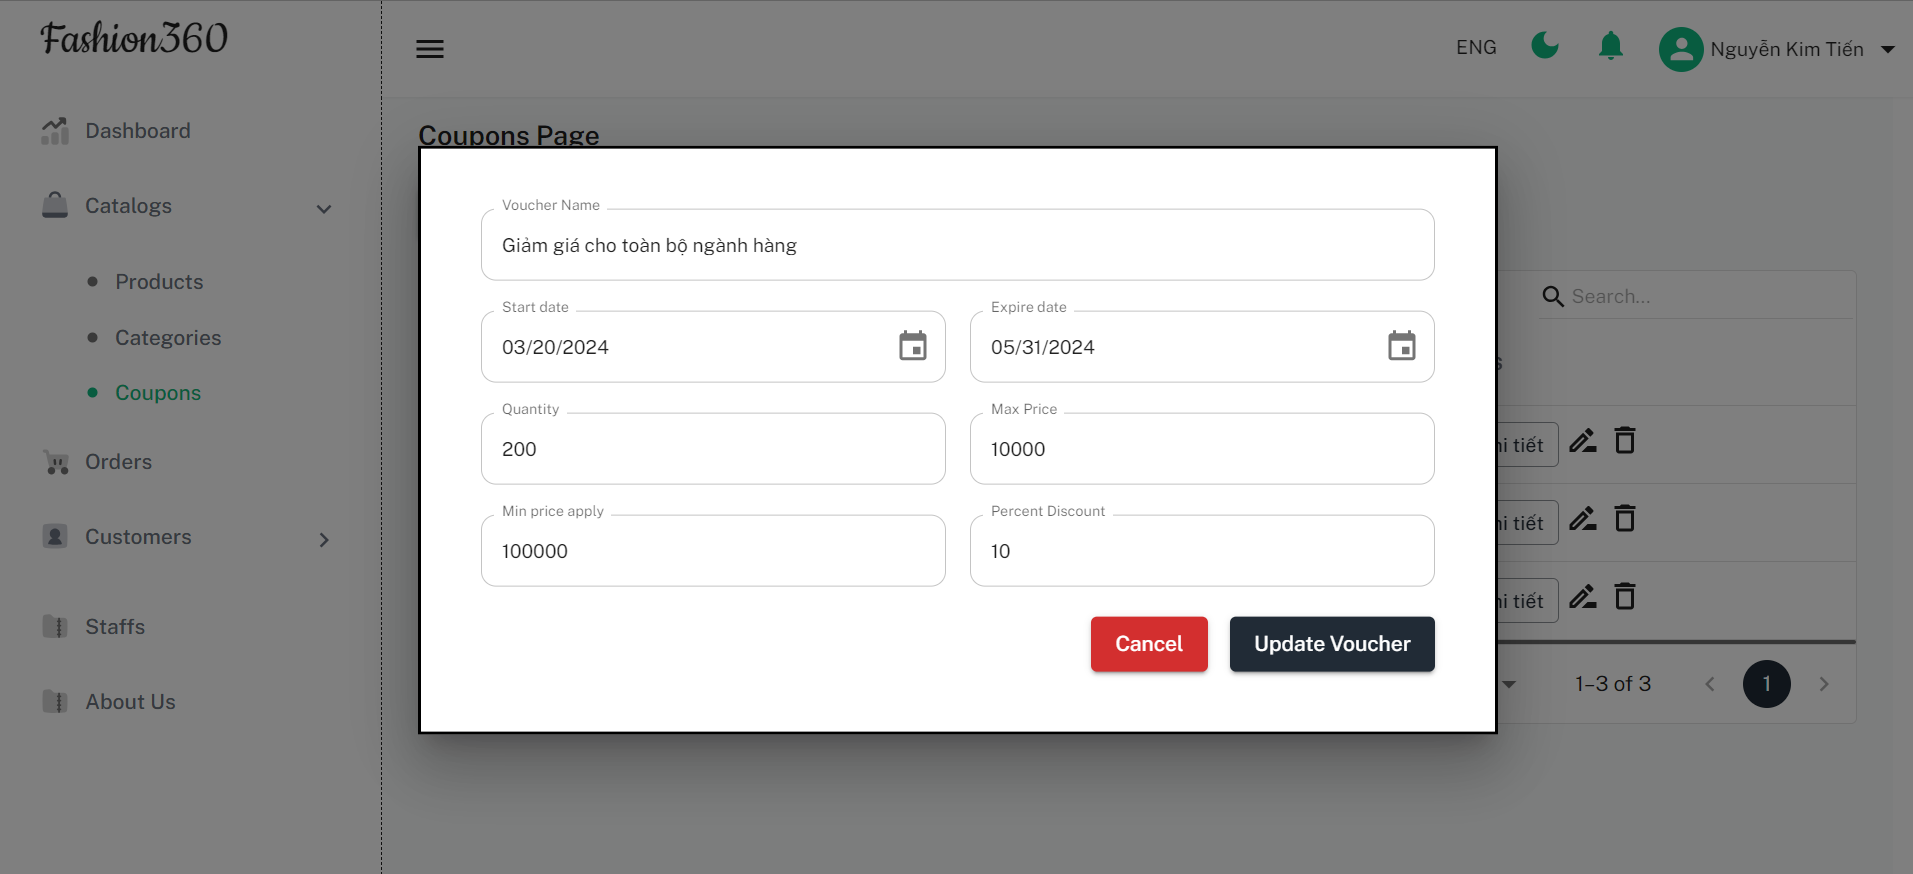
\includegraphics[width=14cm]{Images/Web/updateVoucher.png}
        \newline
        \caption{Giao diện của trang cập nhật mã giảm giá}
\end{figure}
 \begin{figure}[H]
        \centering
        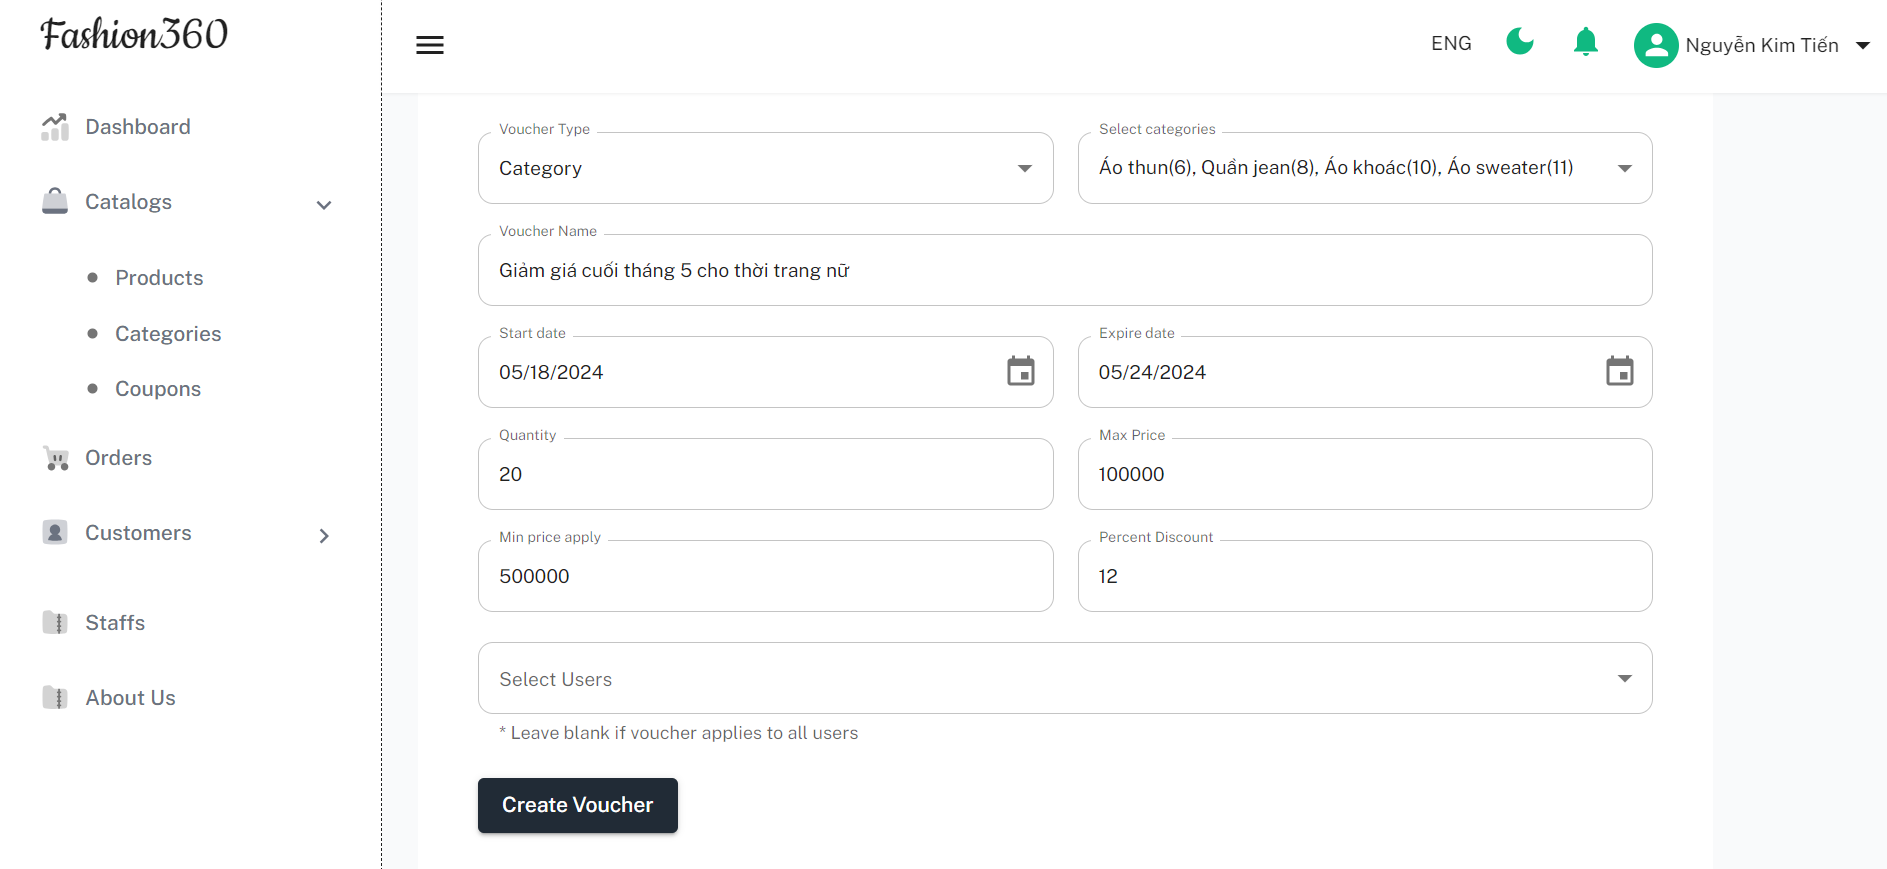
\includegraphics[width=14cm]{Images/Web/addVoucher.png}
        \newline
        \caption{Một phần giao diện của trang tạo mới mã giảm giá}
\end{figure}
 \begin{figure}[H]
        \centering
        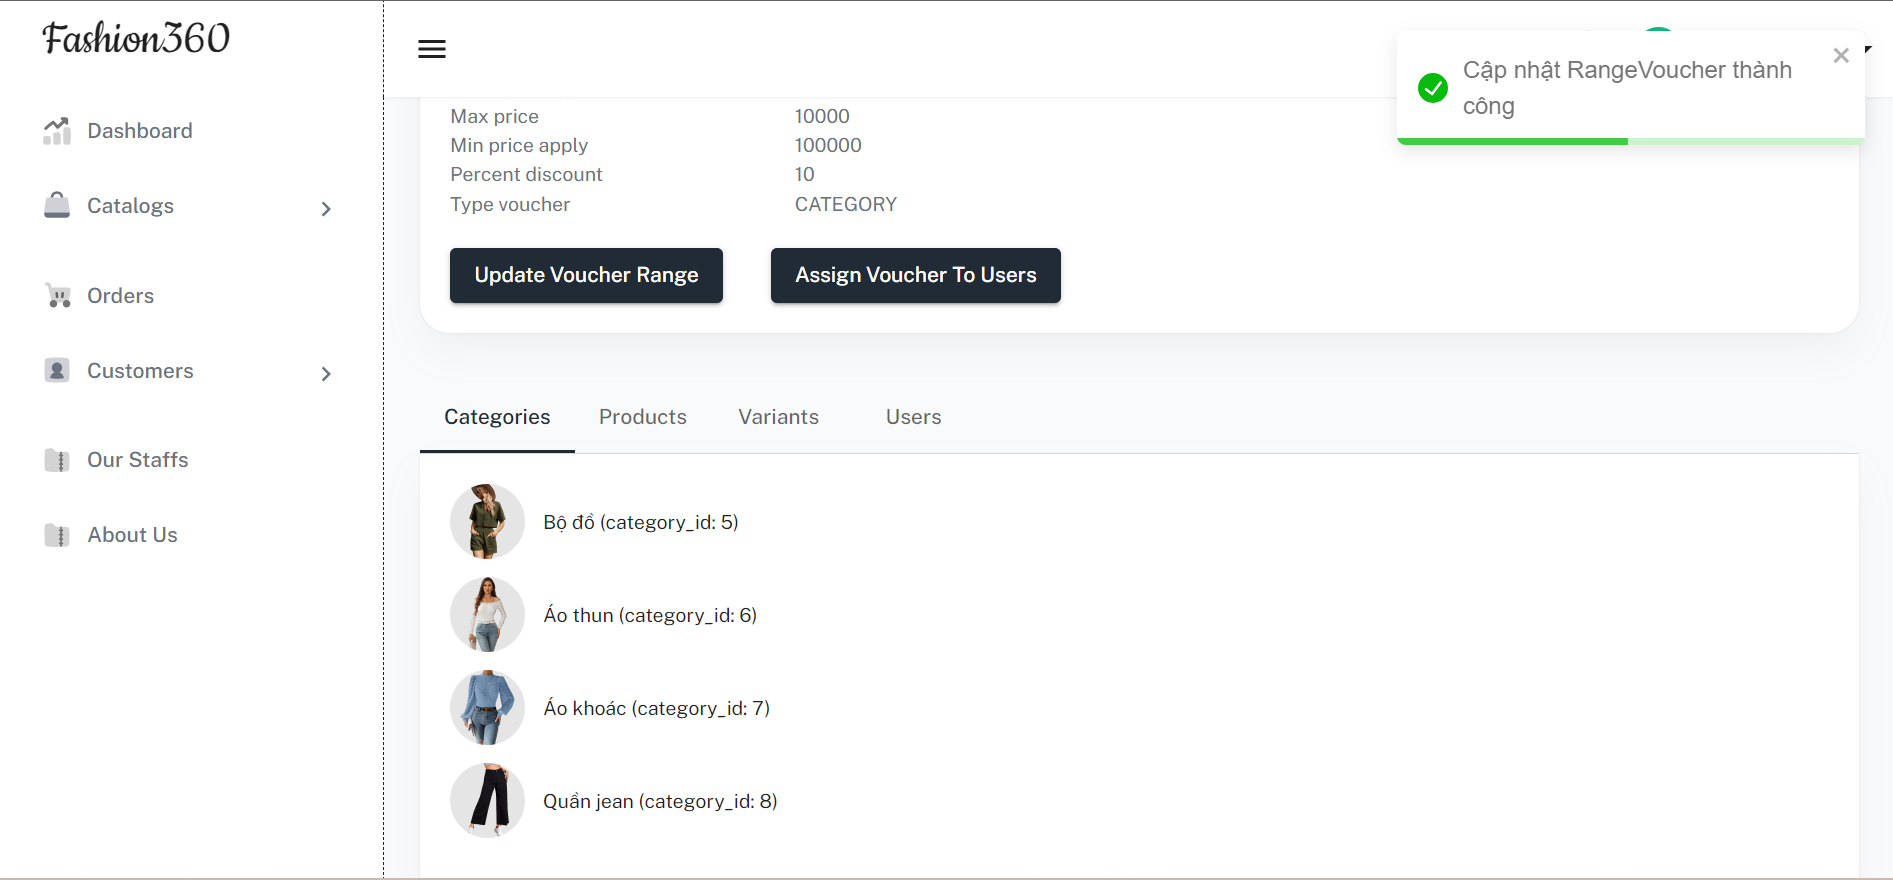
\includegraphics[width=14cm]{Images/Web/updateVoucherCategory.png}
        \newline
        \caption{Một phần giao diện của trang gán mã giảm giá cho thể loại}
\end{figure}
 \begin{figure}[H]
        \centering
        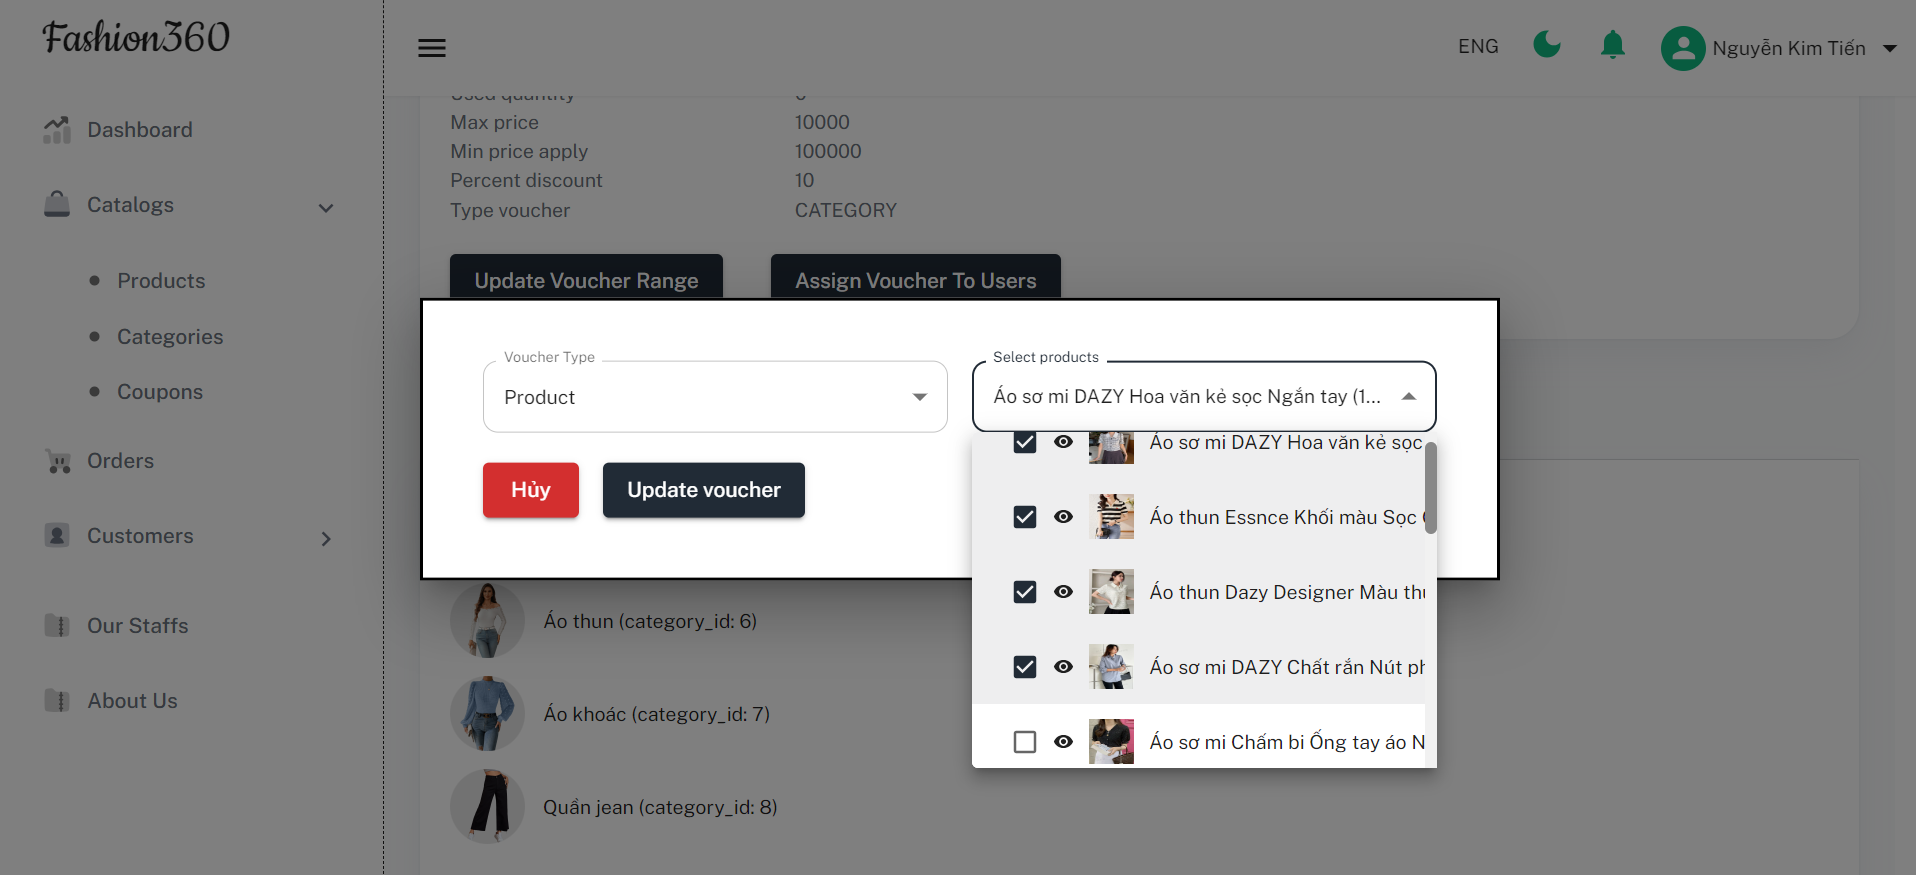
\includegraphics[width=14cm]{Images/Web/updateVoucherProduct.png}
        \newline
        \caption{Một phần giao diện của trang gán mã giảm giá cho sản phẩm}
\end{figure}
\begin{figure}[H]
        \centering
        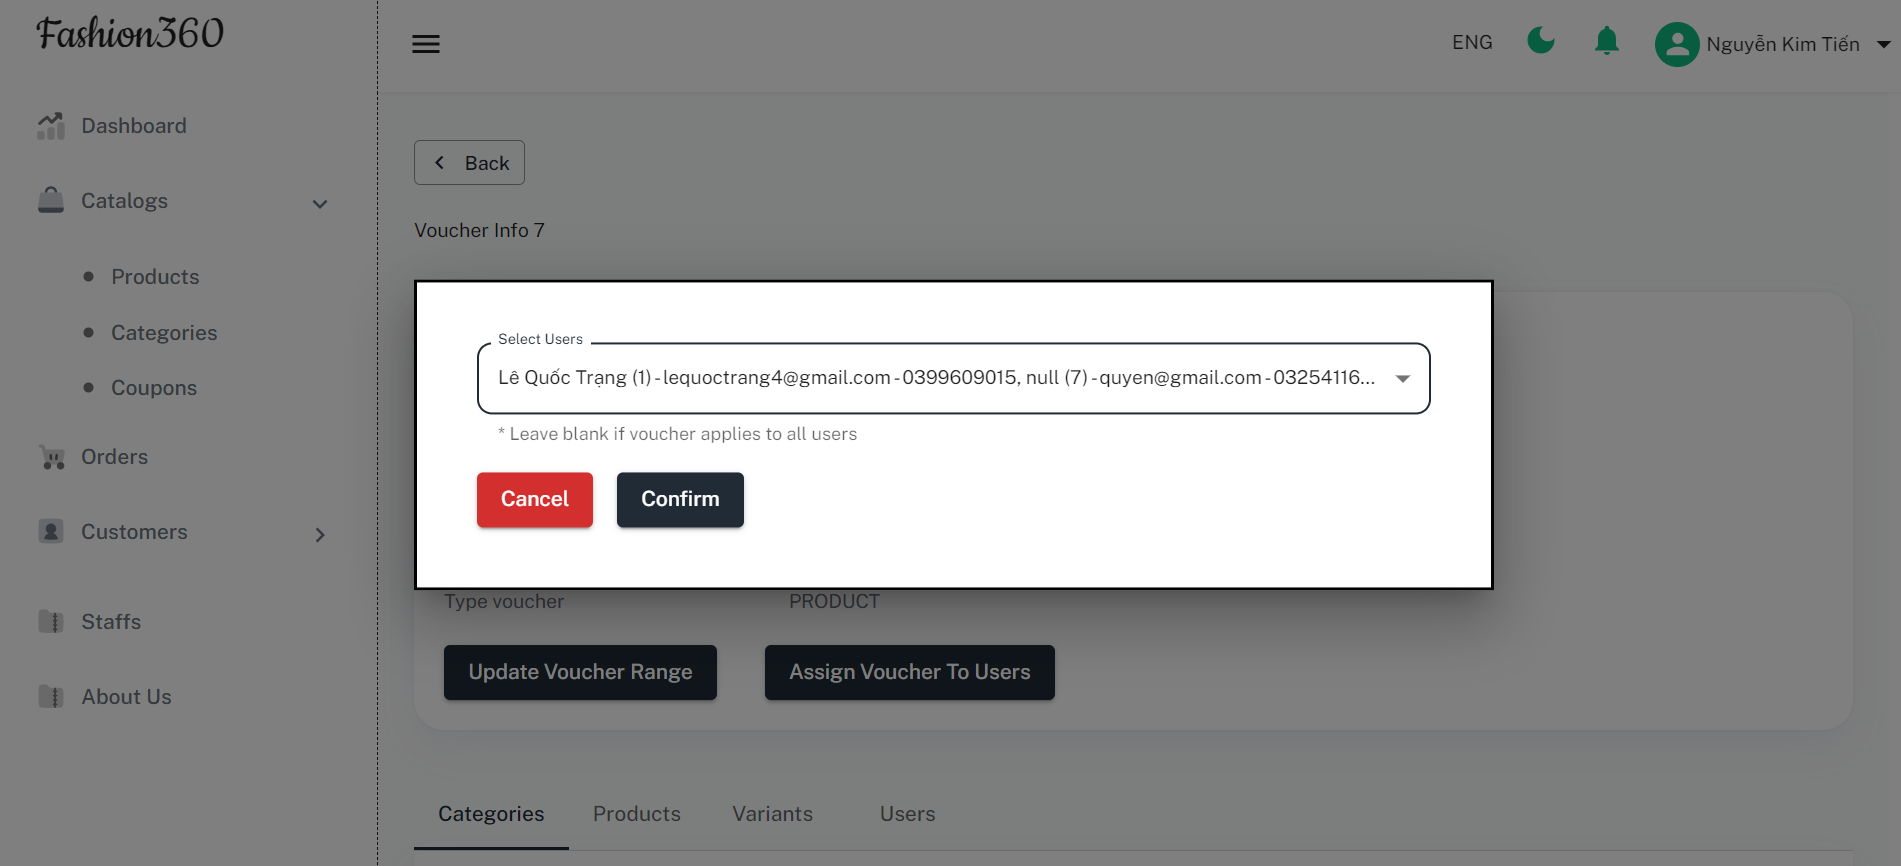
\includegraphics[width=14cm]{Images/Web/updateVoucherUser.png}
        \newline
        \caption{Một phần giao diện của trang gán mã giảm giá cho người dùng}
\end{figure}

\begin{itemize}
    \item \textbf{Trang Đơn hàng (Order)}
\end{itemize}
\begin{figure}[H]
        \centering
        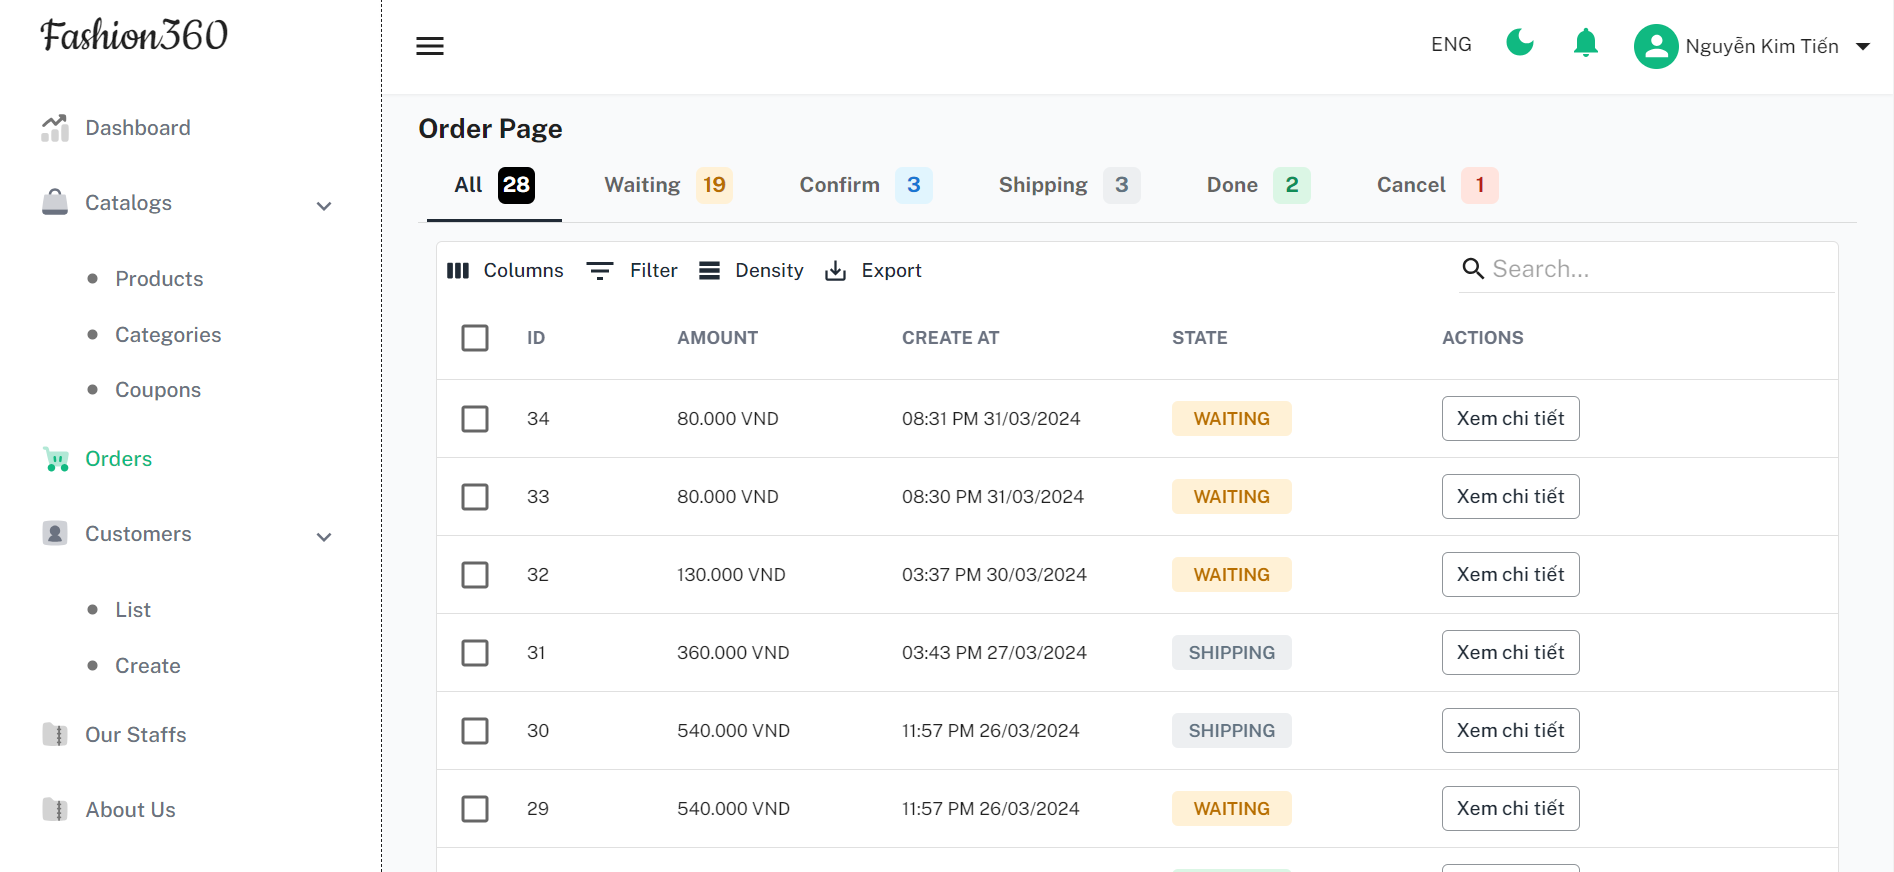
\includegraphics[width=14cm]{Images/Web/order.png}
        \newline
        \caption{Một phần giao diện hiển thị danh sách đơn hàng}
\end{figure}
\begin{figure}[H]
        \centering
        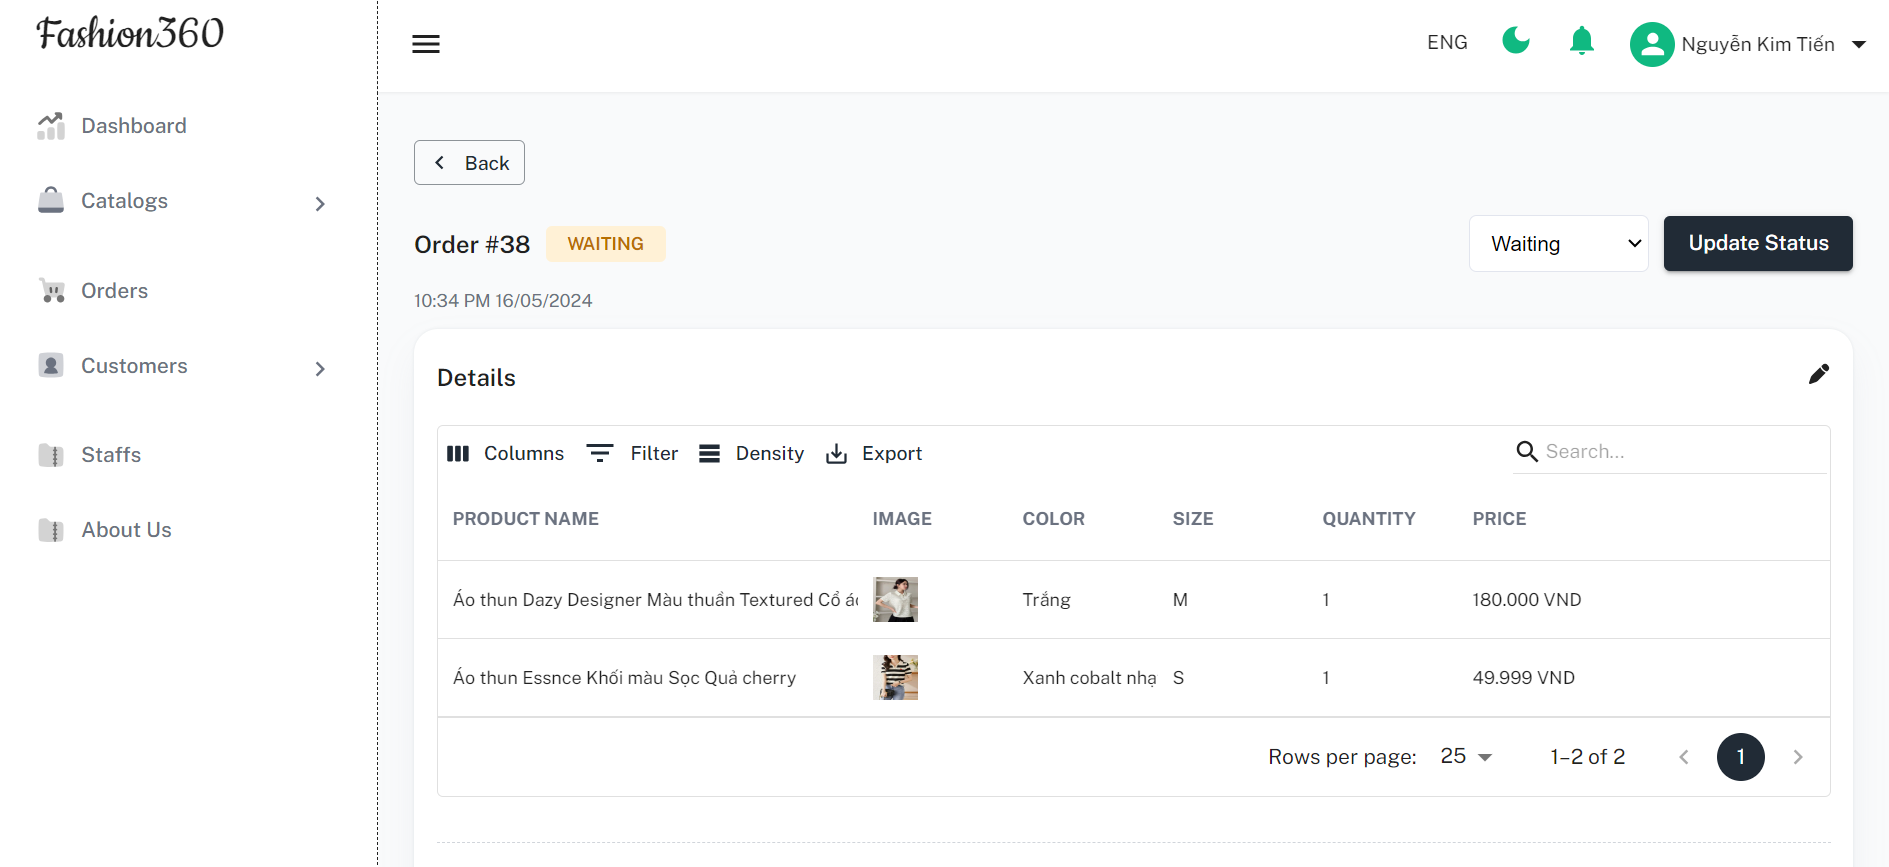
\includegraphics[width=14cm]{Images/Web/orderDetail1.png}
        \newline
        \caption{Một phần giao diện hiển thị thông tin chi tiết đơn hàng}
\end{figure}
\begin{figure}[H]
        \centering
        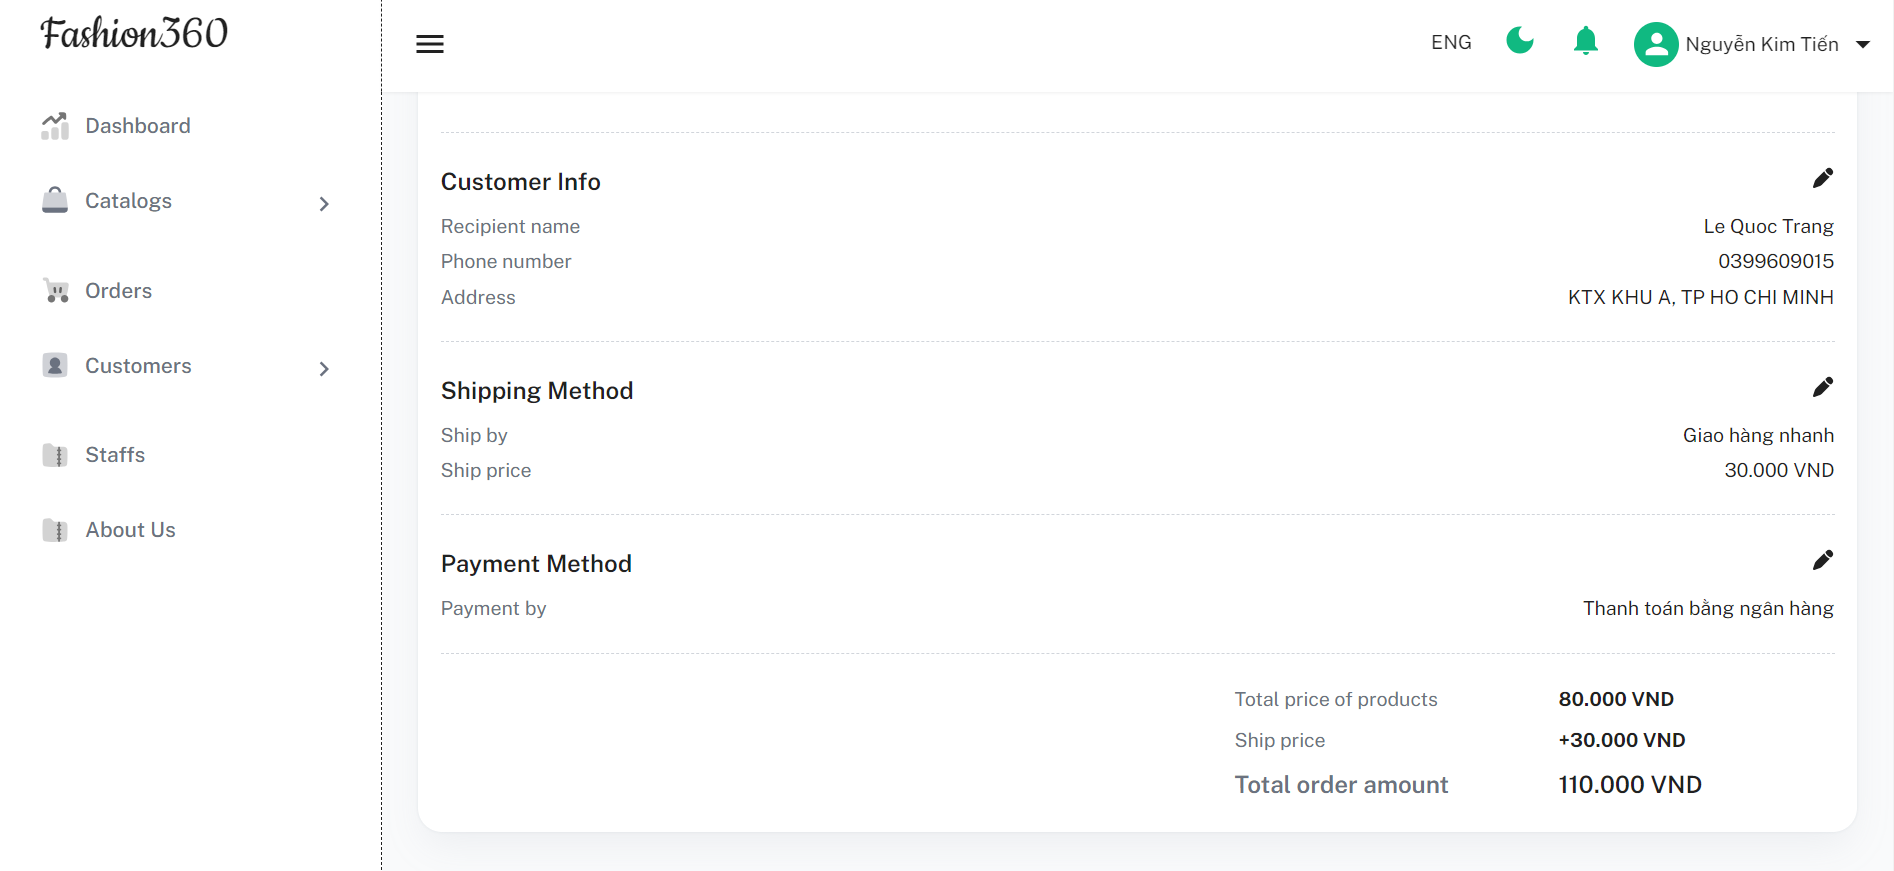
\includegraphics[width=14cm]{Images/Web/orderDetail2.png}
        \newline
        \caption{Một phần giao diện hiển thị thông tin chi tiết đơn hàng}
\end{figure}

\begin{itemize}
    \item \textbf{Trang Khách hàng (Customer)}
\end{itemize}

\begin{figure}[H]
        \centering
        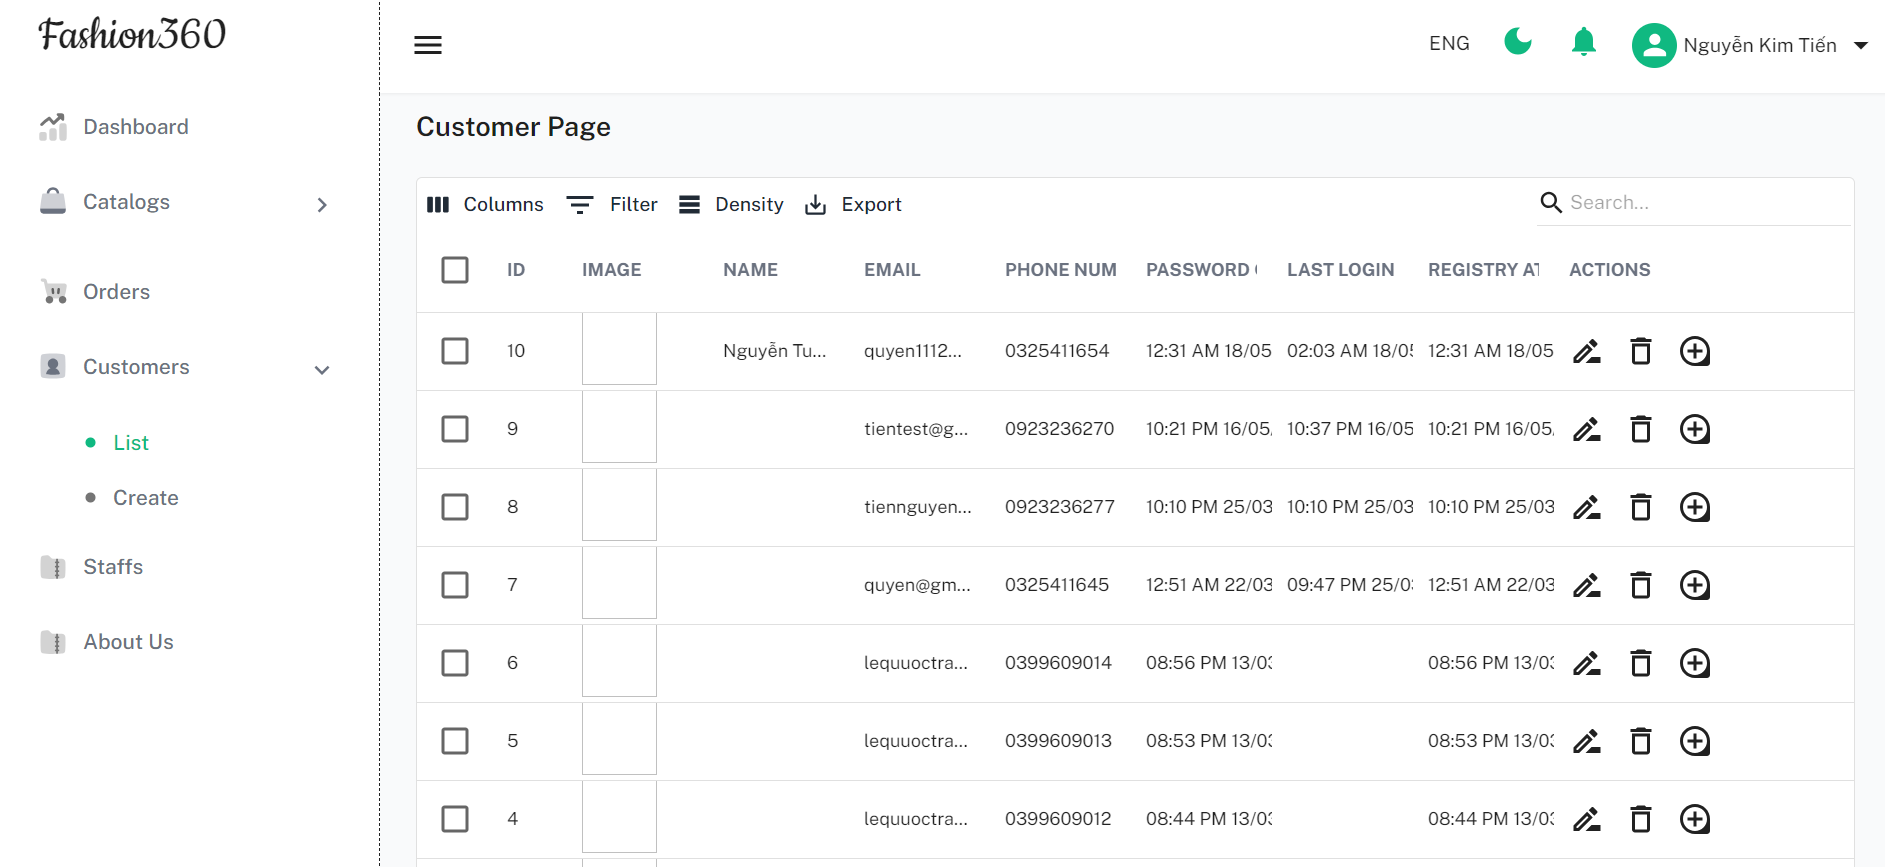
\includegraphics[width=14cm]{Images/Web/CustomerList.png}
        \newline
        \caption{Giao diện hiển thị danh sách khách hàng}
\end{figure}

\begin{figure}[H]
        \centering
        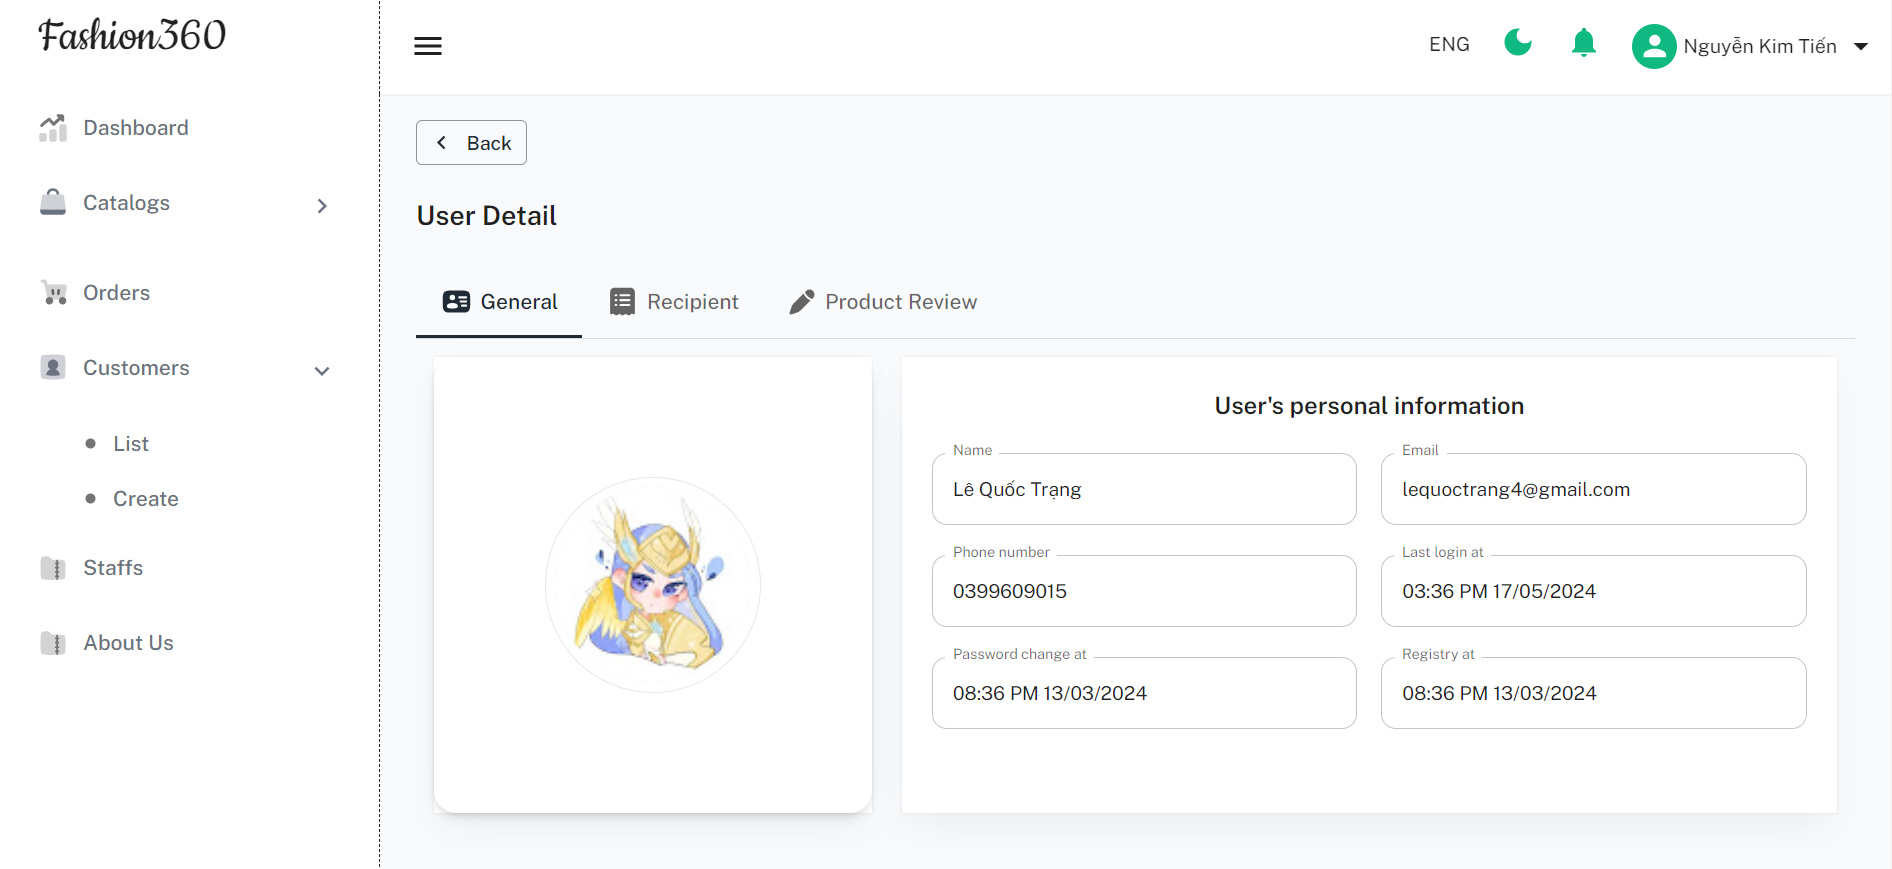
\includegraphics[width=14cm]{Images/Web/userDetail1.png}
        \newline
        \caption{Giao diện hiển thị thông tin cá nhân của khách hàng}
\end{figure}

\begin{figure}[H]
        \centering
        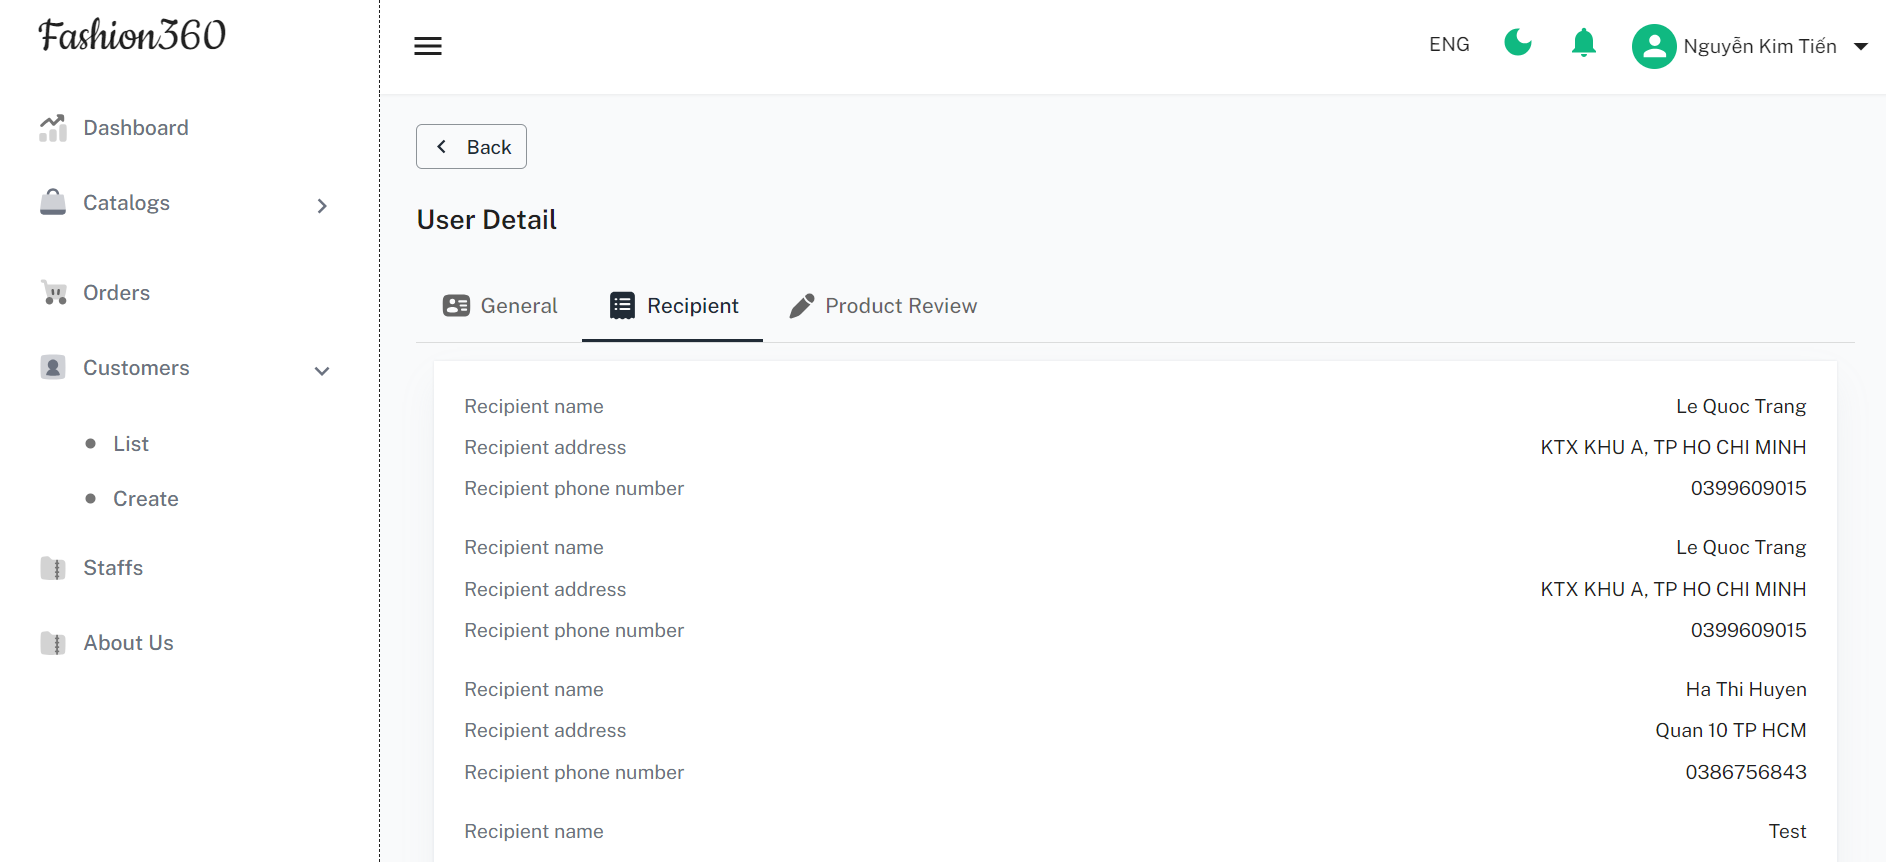
\includegraphics[width=14cm]{Images/Web/userDetail2.png}
        \newline
        \caption{Giao diện hiển thị thông tin nhận hàng của khách hàng}
\end{figure}

\begin{itemize}
    \item \textbf{Trang Nhân viên (Staff)}
\end{itemize}
\begin{figure}[H]
        \centering
        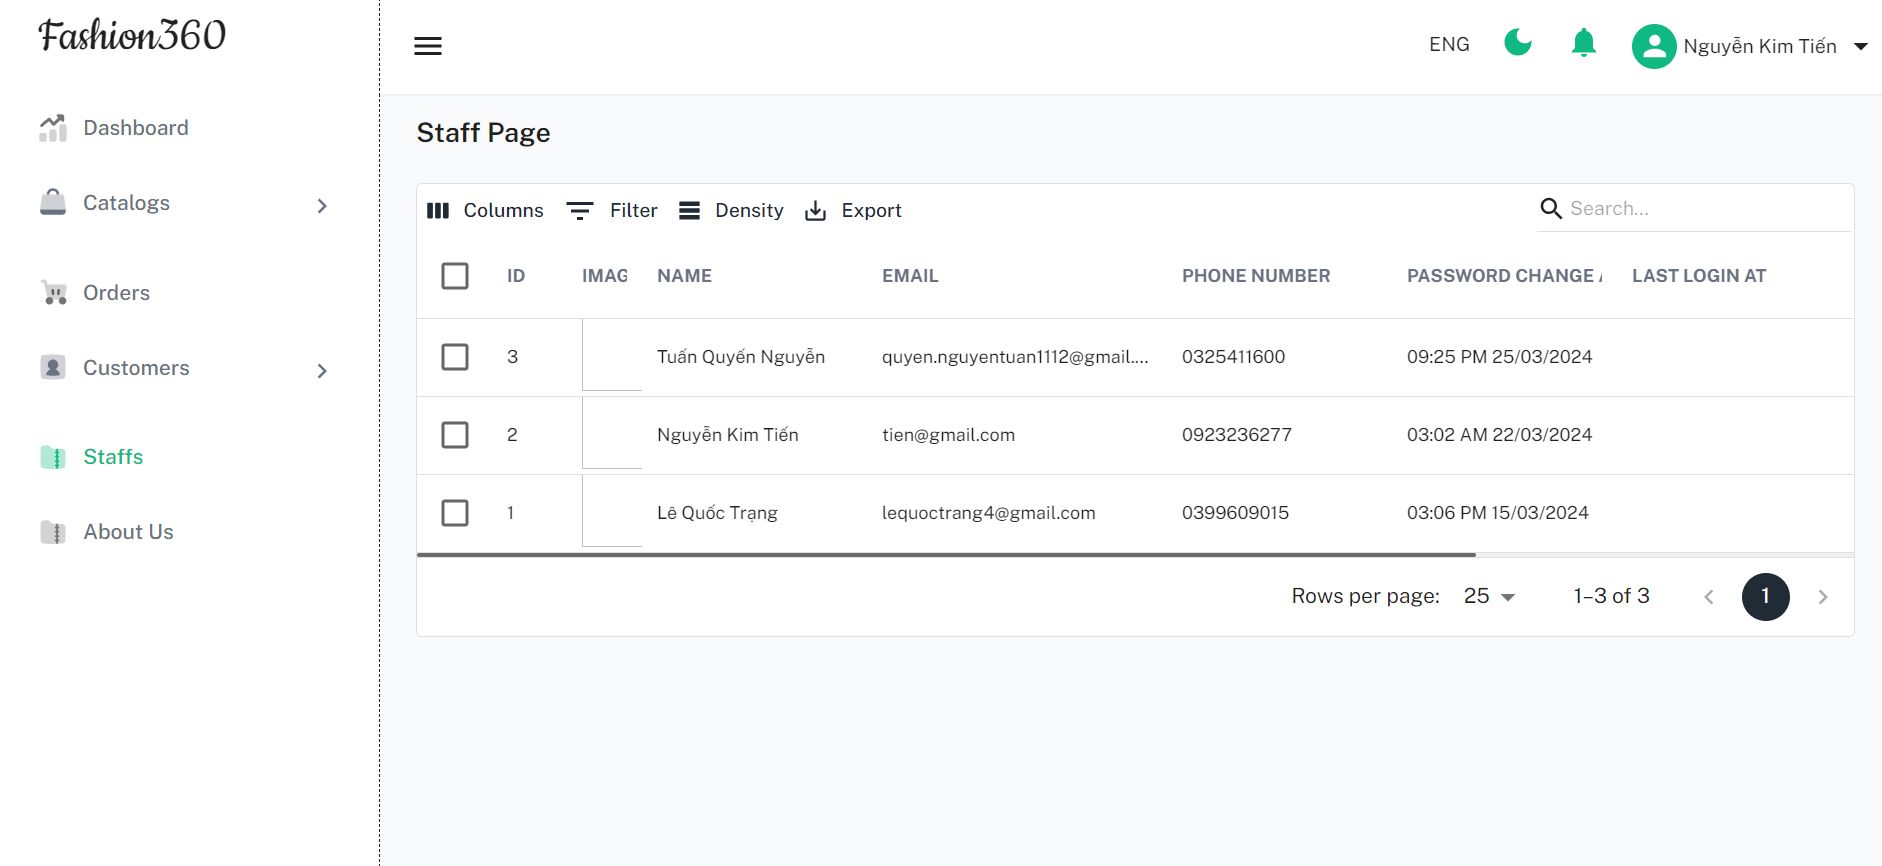
\includegraphics[width=14cm]{Images/Web/staffList.png}
        \newline
        \caption{Giao diện hiển thị danh sách nhân viên}
\end{figure}
\begin{figure}[H]
        \centering
        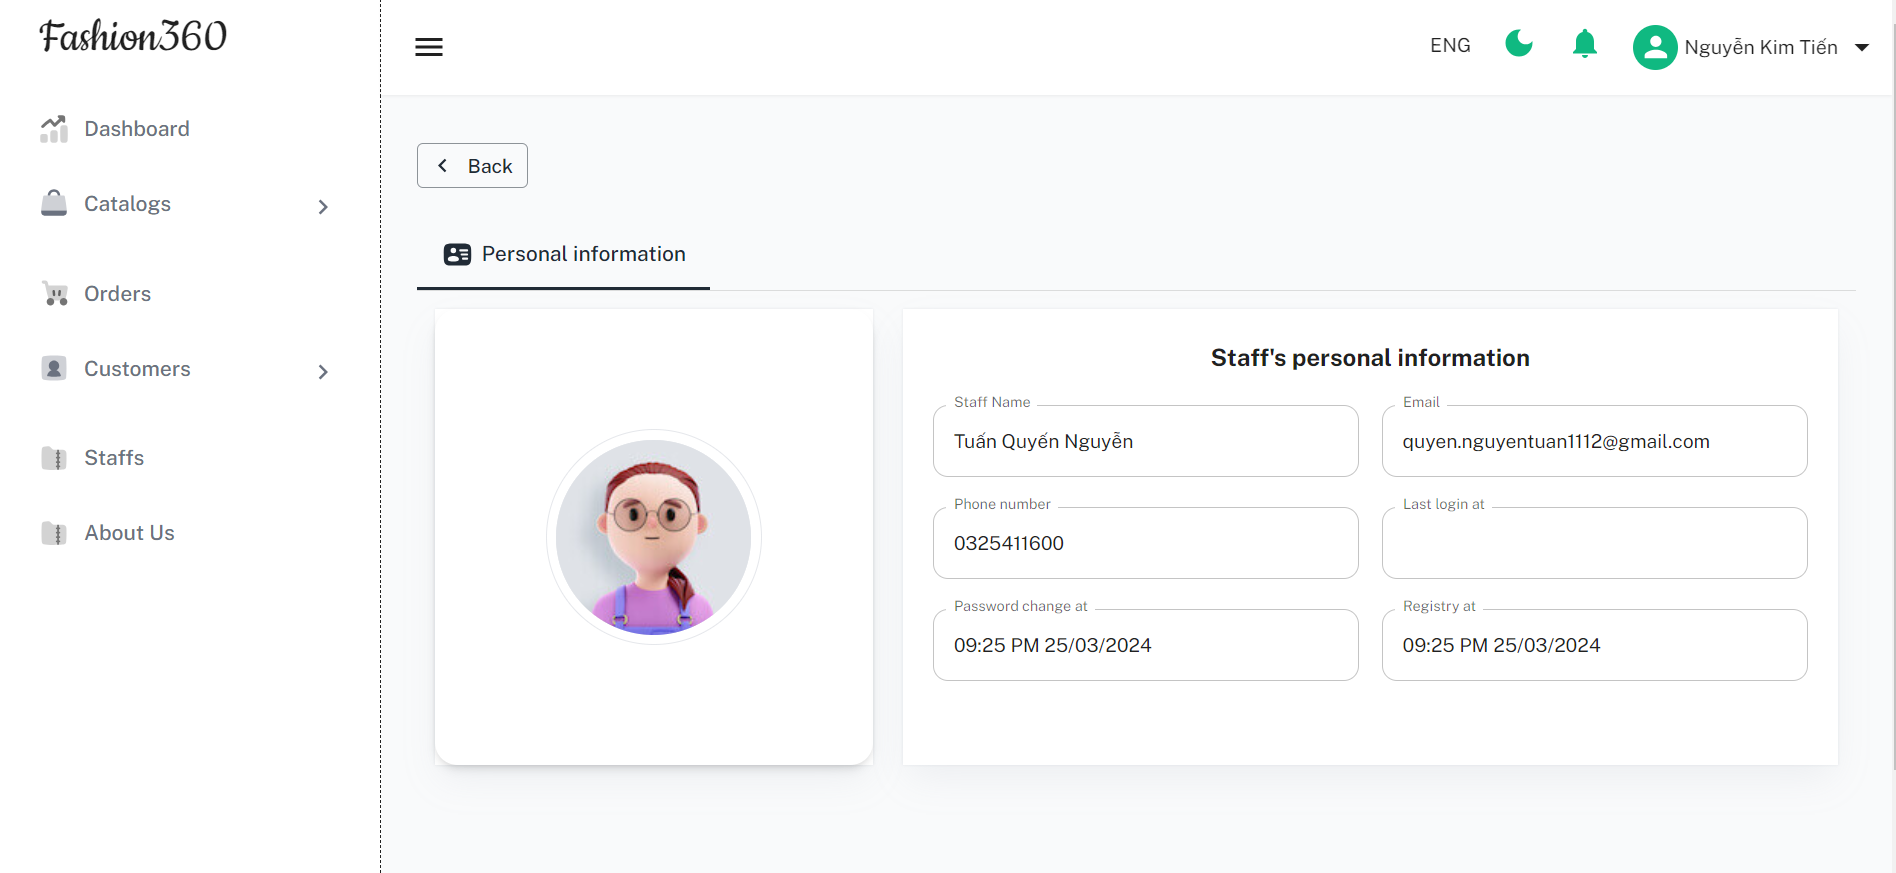
\includegraphics[width=14cm]{Images/Web/staffDetail.png}
        \newline
        \caption{Giao diện hiển thị thông tin cá nhân của nhân viên}
\end{figure}

\subsubsection{Giao diện ứng dụng di động của người dùng}

    \begin{figure}[H]
    \centering
    \begin{minipage}{0.45\textwidth}
        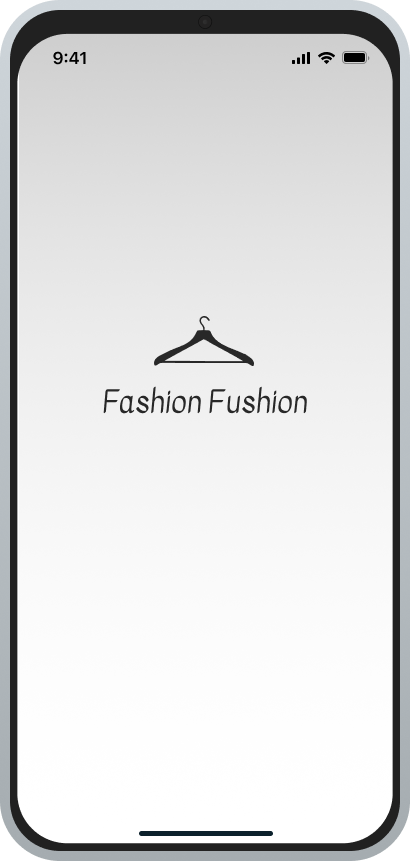
\includegraphics[scale=0.35]{Images/Design/User/GettingStarted/Launch screem.png}
        \vspace{10pt}
        \centering
        \caption{Khởi động ứng dụng}
    \end{minipage}\hfill
    \begin{minipage}{0.45\textwidth}
        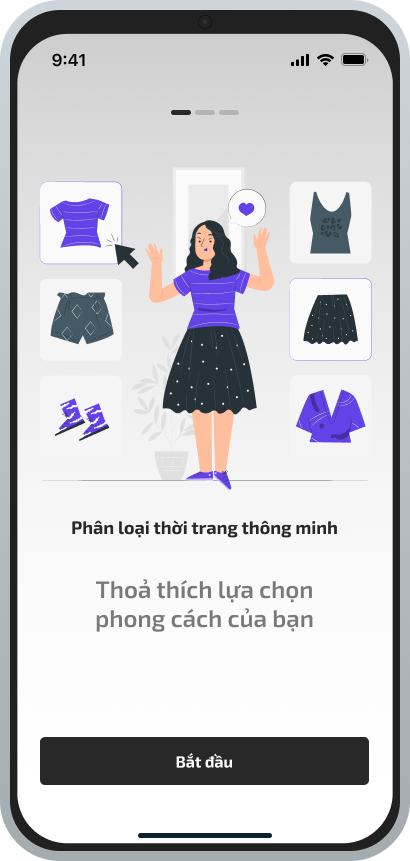
\includegraphics[scale=0.35]{Images/Design/User/GettingStarted/Onboarding.png}
        \vspace{10pt}
        \centering
        \caption{Giới thiệu}
    \end{minipage}
    \end{figure}

     \begin{figure}[H]
    \centering
    \begin{minipage}{0.45\textwidth}
        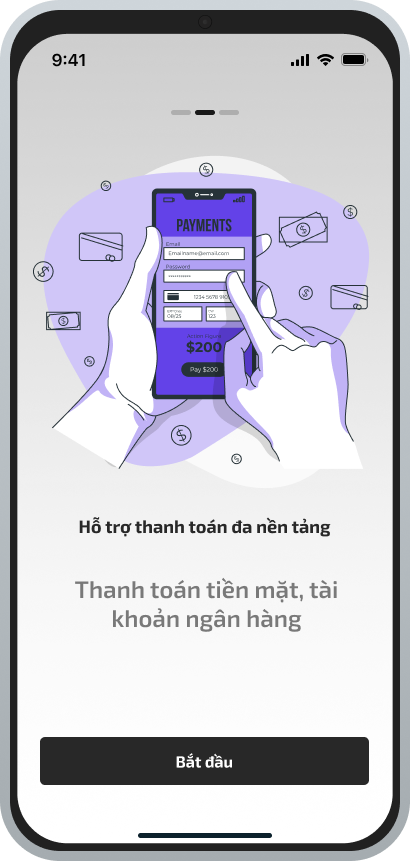
\includegraphics[scale=0.35]{Images/Design/User/GettingStarted/Onboarding (1).png}
        \vspace{10pt}
        \centering
        \caption{Giới thiệu}
    \end{minipage}\hfill
    \begin{minipage}{0.45\textwidth}
        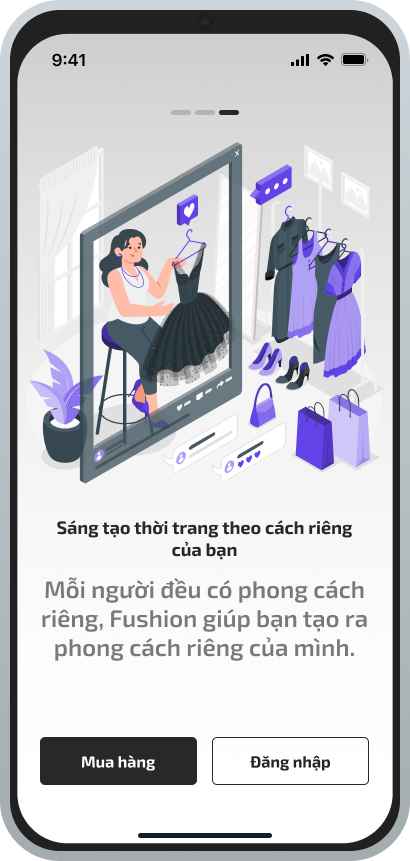
\includegraphics[scale=0.35]{Images/Design/User/GettingStarted/Get started.png}
        \vspace{10pt}
        \centering
        \caption{Giới thiệu}
    \end{minipage}
    \end{figure}

    % Author

      \begin{figure}[H]
    \centering
    \begin{minipage}{0.45\textwidth}
        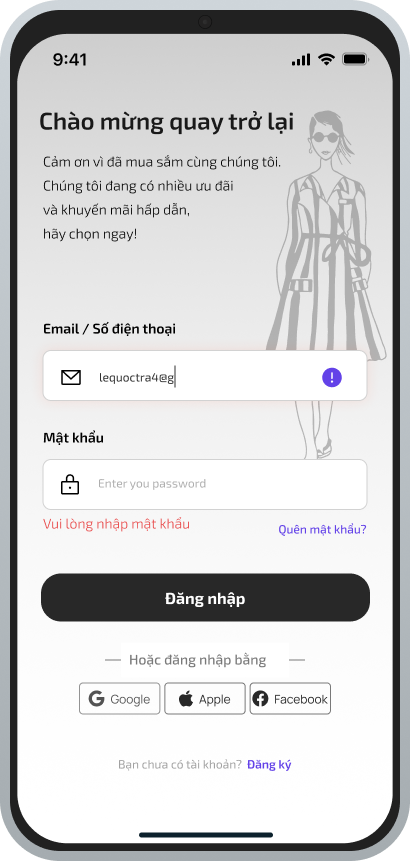
\includegraphics[scale=0.35]{Images/Design/User/Author/SignIn.png}
        \vspace{10pt}
        \centering \caption{Đăng nhập}
    \end{minipage}\hfill
    \begin{minipage}{0.45\textwidth}
        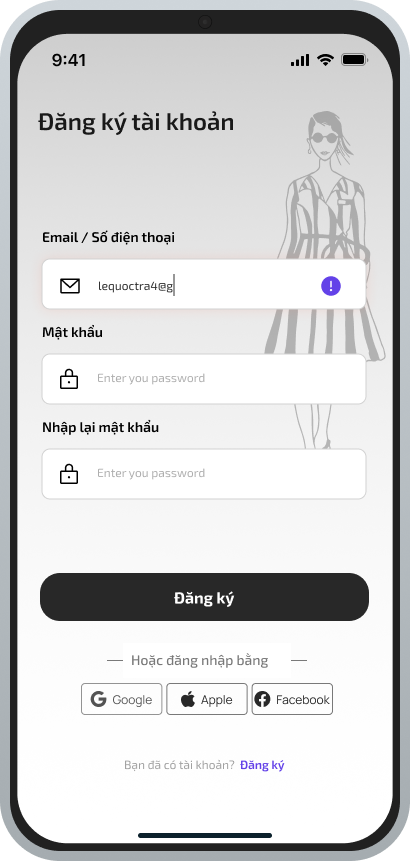
\includegraphics[scale=0.35]{Images/Design/User/Author/SignUp.png}
        \vspace{10pt}
        \centering \caption{Đăng ký tài khoản}
    \end{minipage}
    \end{figure}

      \begin{figure}[H]
    \centering
    \begin{minipage}{0.45\textwidth}
        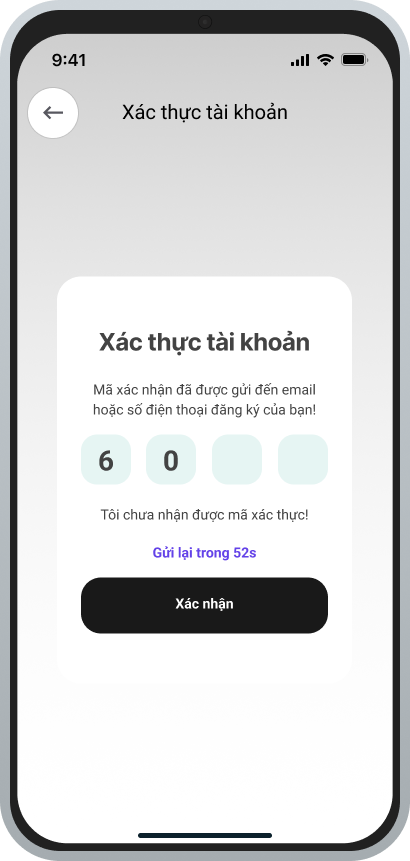
\includegraphics[scale=0.35]{Images/Design/User/Author/Xác thực.png}
        \vspace{10pt}
        \centering \caption{Nhập mã xác thực tài khoản}
    \end{minipage}\hfill
    \begin{minipage}{0.45\textwidth}
        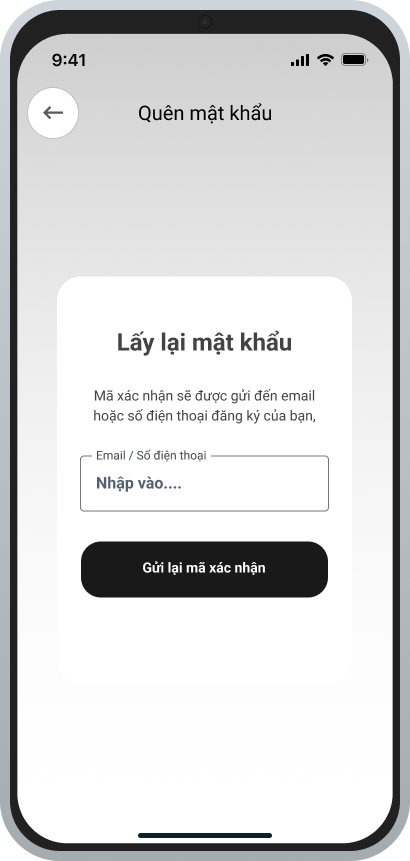
\includegraphics[scale=0.35]{Images/Design/User/Author/Quên mật khẩu.png}
        \vspace{10pt}
        \centering \caption{Lấy lại mật khẩu}
    \end{minipage}
    \end{figure}

      \begin{figure}[H]
    \centering
    \begin{minipage}{0.45\textwidth}
        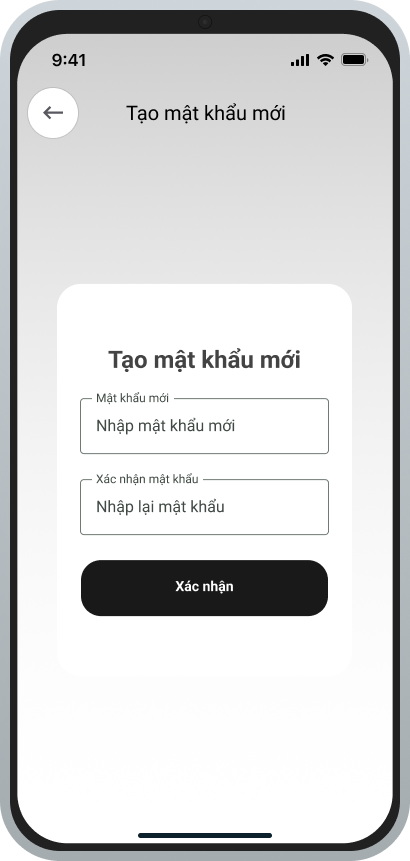
\includegraphics[scale=0.35]{Images/Design/User/Author/Tạo mật khẩu mới 1.png}
        \vspace{10pt}
        \centering \caption{Tạo mật khẩu mới}
    \end{minipage}\hfill
    \begin{minipage}{0.45\textwidth}
        \includegraphics[width=5cm]{{Images/Design/User/Main/Search.png}}
        \vspace{10pt}
        \centering \caption{Tìm kiếm sản phẩm}
    \end{minipage}
    \end{figure}


    \begin{figure}[H]
    \centering
    \begin{minipage}{0.45\textwidth}
        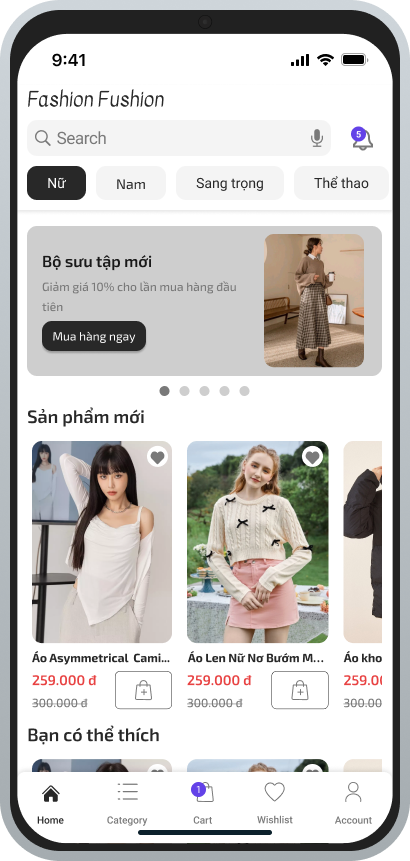
\includegraphics[scale=0.35]{Images/Design/User/Main/HomePage.png}
        \vspace{10pt}
        \centering \caption{Trang chủ}
    \end{minipage}\hfill
    \begin{minipage}{0.45\textwidth}
        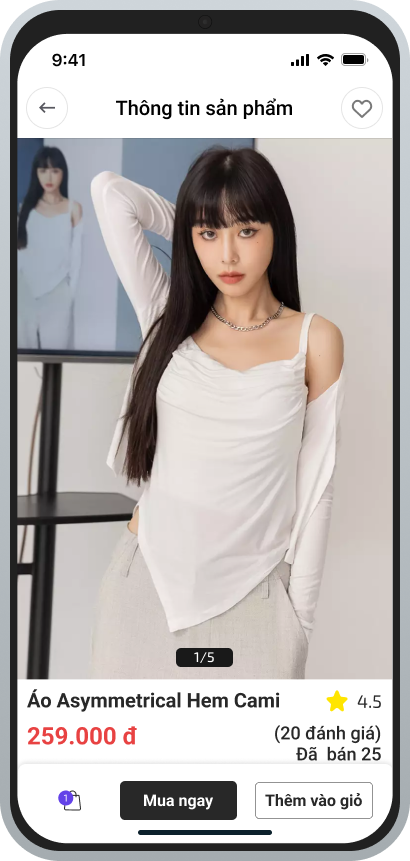
\includegraphics[scale=0.35]{Images/Design/User/Main/Product Detail.png}
        \vspace{10pt}
        \centering \caption{Thông tin sản phẩm}
    \end{minipage}
    \end{figure}

      \begin{figure}[H]
    \centering
    \begin{minipage}{0.45\textwidth}
        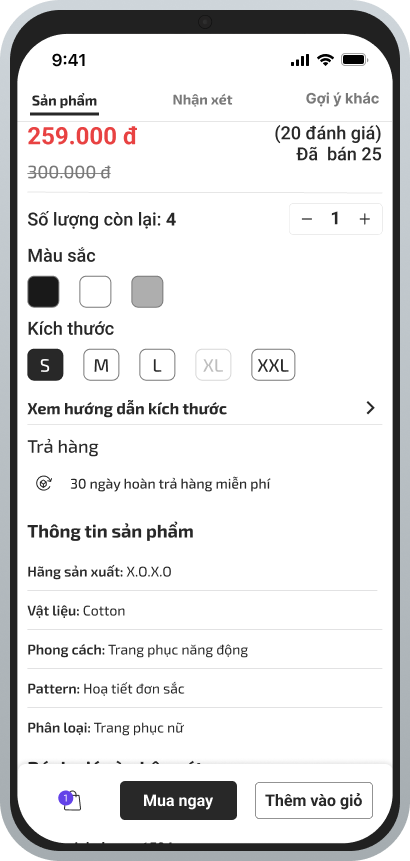
\includegraphics[scale=0.35]{Images/Design/User/Main/Product Detail-1.png}
        \vspace{10pt}
        \centering \caption{Thông tin chi tiết sản phẩm}
    \end{minipage}\hfill
    \begin{minipage}{0.45\textwidth}
        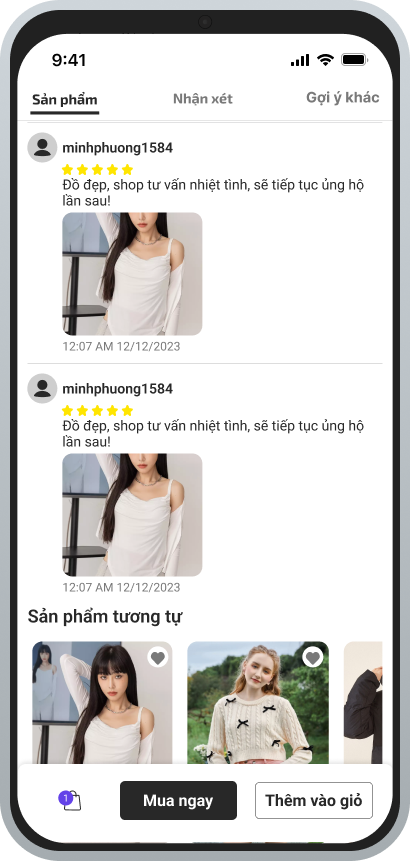
\includegraphics[scale=0.35]{Images/Design/User/Main/Product Detail-2.png}
        \vspace{10pt}
        \centering \caption{Xem đánh giá về sản phẩm}
    \end{minipage}
    \end{figure}

      \begin{figure}[H]
    \centering
    \begin{minipage}{0.45\textwidth}
        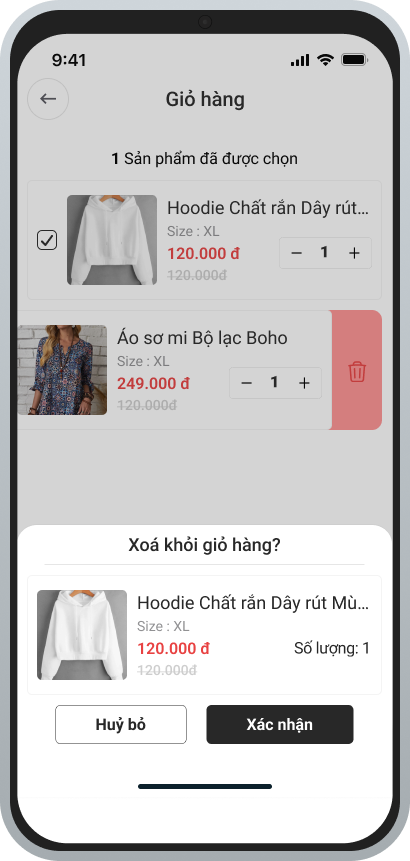
\includegraphics[scale=0.35]{Images/Design/User/Main/Giỏ hàng.png}
        \vspace{10pt}
        \centering \caption{Xóa sản phẩm khỏi giỏ hàng}
    \end{minipage}\hfill
    \begin{minipage}{0.45\textwidth}
        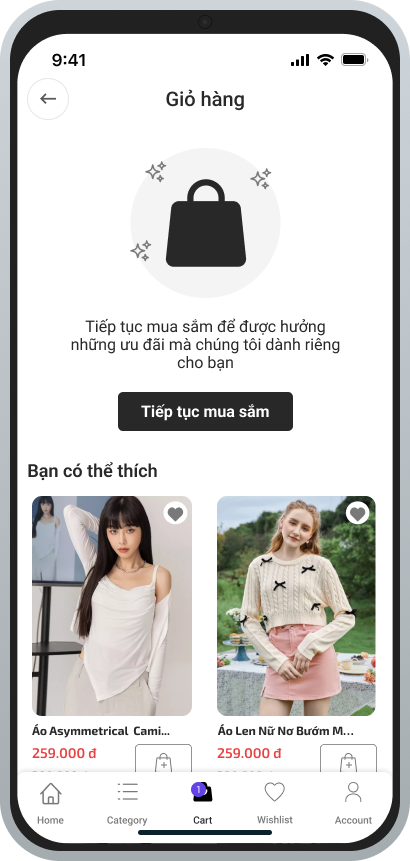
\includegraphics[scale=0.35]{Images/Design/User/Main/Giỏ hàng-1.png}
        \vspace{10pt}
        \centering \caption{Xem giỏ hàng}
    \end{minipage}
    \end{figure}

      \begin{figure}[H]
    \centering
    \begin{minipage}{0.45\textwidth}
        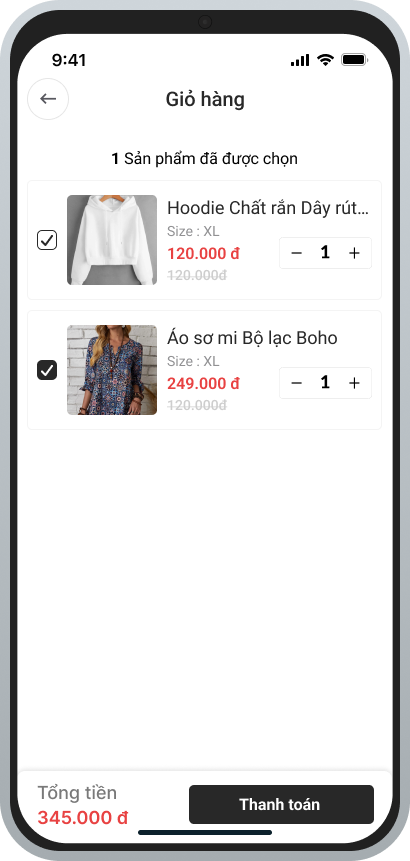
\includegraphics[scale=0.35]{Images/Design/User/Main/Giỏ hàng-2.png}
        \vspace{10pt}
        \centering \caption{Chỉnh sửa giỏ hàng }
    \end{minipage}\hfill
    \begin{minipage}{0.45\textwidth}
        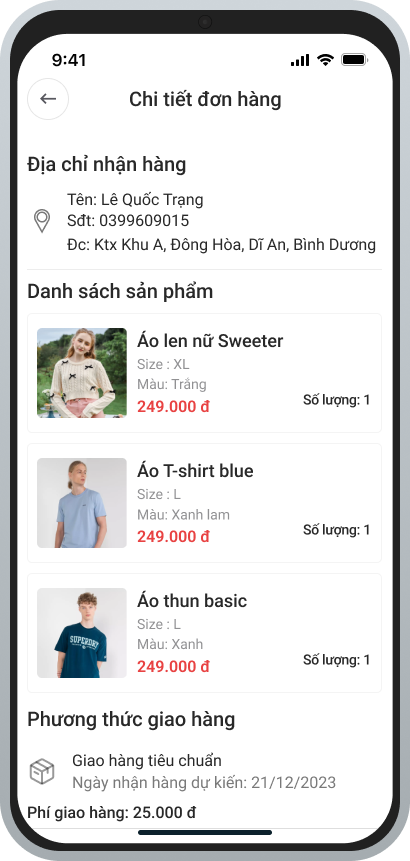
\includegraphics[scale=0.35]{Images/Design/User/Main/Order detail.png}
        \vspace{10pt}
        \centering \caption{Chi tiết đơn hàng}
    \end{minipage}
    \end{figure}

      \begin{figure}[H]
    \centering
    \begin{minipage}{0.45\textwidth}
        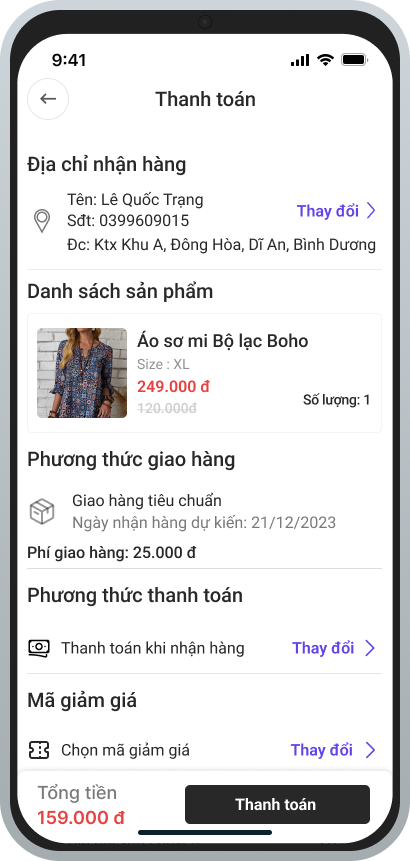
\includegraphics[scale=0.35]{Images/Design/User/Main/Thanh toán.png}
        \vspace{10pt}
        \centering \caption{Thanh toán đơn hàng}
    \end{minipage}\hfill
    \begin{minipage}{0.45\textwidth}
        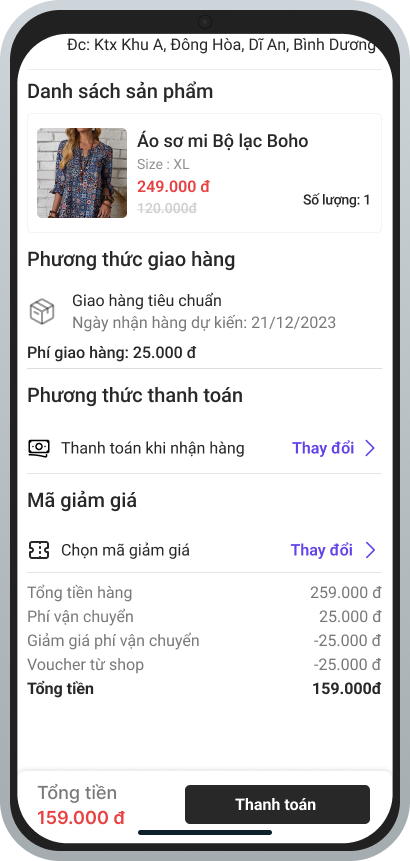
\includegraphics[scale=0.35]{Images/Design/User/Main/Thanh toán-1.png}
        \vspace{10pt}
        \centering \caption{Thanh toán đơn hàng}
    \end{minipage}
    \end{figure}

      \begin{figure}[H]
    \centering
    \begin{minipage}{0.45\textwidth}
        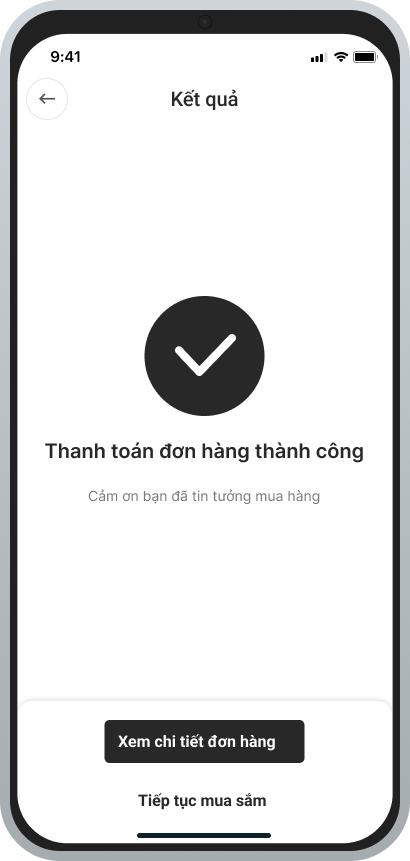
\includegraphics[scale=0.35]{Images/Design/User/Main/Payment Success.png}
        \vspace{10pt}
        \centering \caption{Thanh toán đơn hàng thành công}
    \end{minipage}\hfill
    \begin{minipage}{0.45\textwidth}
        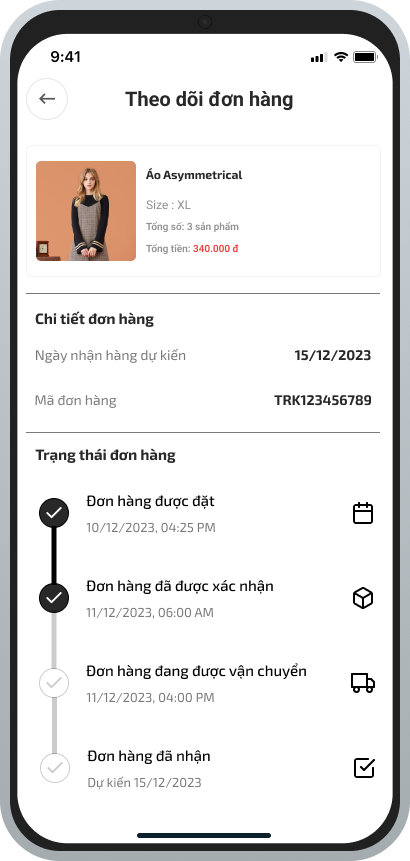
\includegraphics[scale=0.35]{Images/Design/User/Main/Track order.png}
        \vspace{10pt}
        \centering \caption{Theo dõi đơn hàng}
    \end{minipage}
    \end{figure}

      \begin{figure}[H]
    \centering
    \begin{minipage}{0.45\textwidth}
        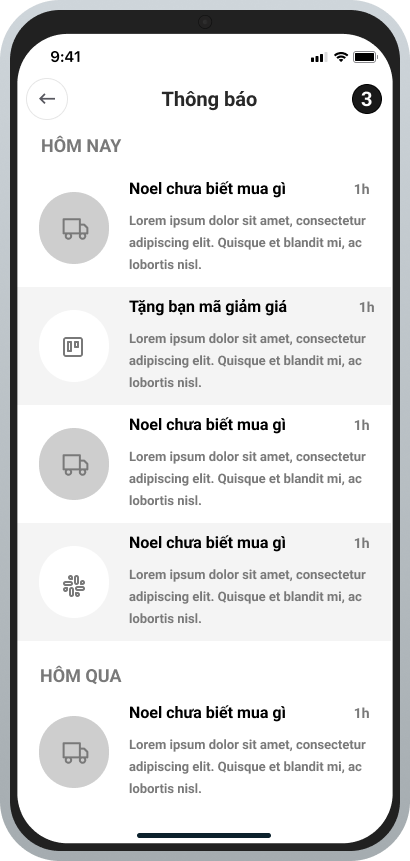
\includegraphics[scale=0.35]{Images/Design/User/Main/Thông báo.png}
        \vspace{10pt}
        \centering \caption{Xem thông báo}
    \end{minipage}\hfill
    \begin{minipage}{0.45\textwidth}
        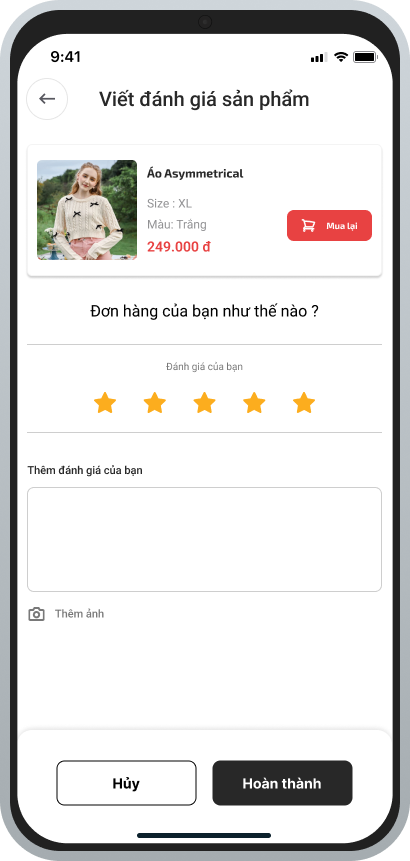
\includegraphics[scale=0.35]{Images/Design/User/Main/Viết đánh giá.png}
        \vspace{10pt}
        \centering \caption{Viết đánh giá sản phẩm}
    \end{minipage}
    \end{figure}

      \begin{figure}[H]
    \centering
    \begin{minipage}{0.45\textwidth}
        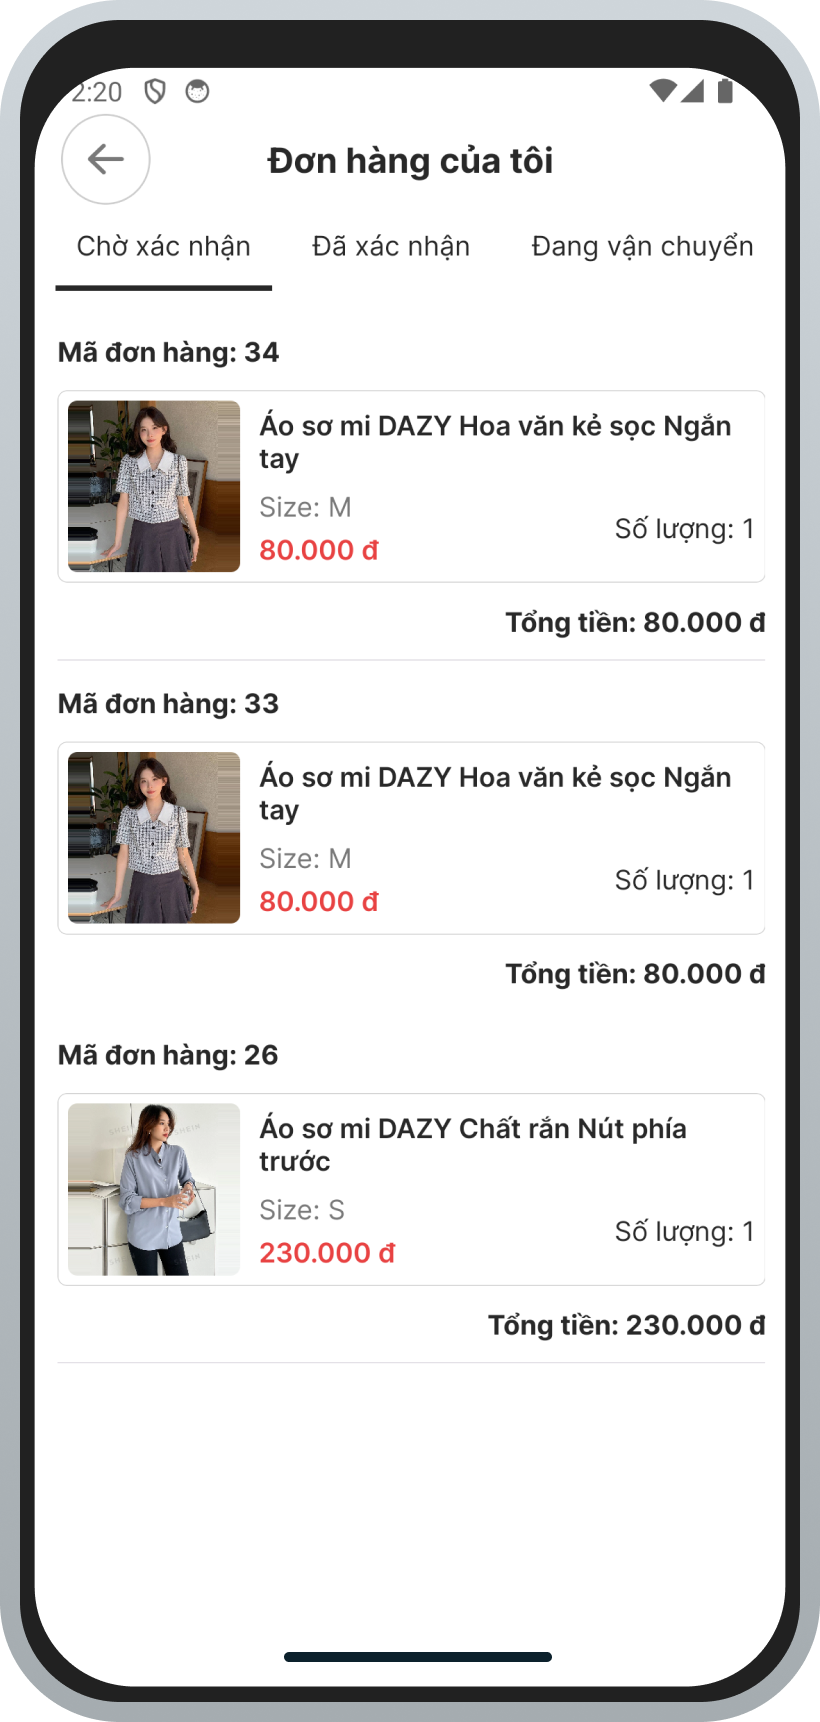
\includegraphics[width=5cm]{Images/Design/User/Main/order-status.png}
        \vspace{10pt}
        \centering \caption{Trạng thái đơn hàng}
    \end{minipage}\hfill
    \begin{minipage}{0.45\textwidth}
 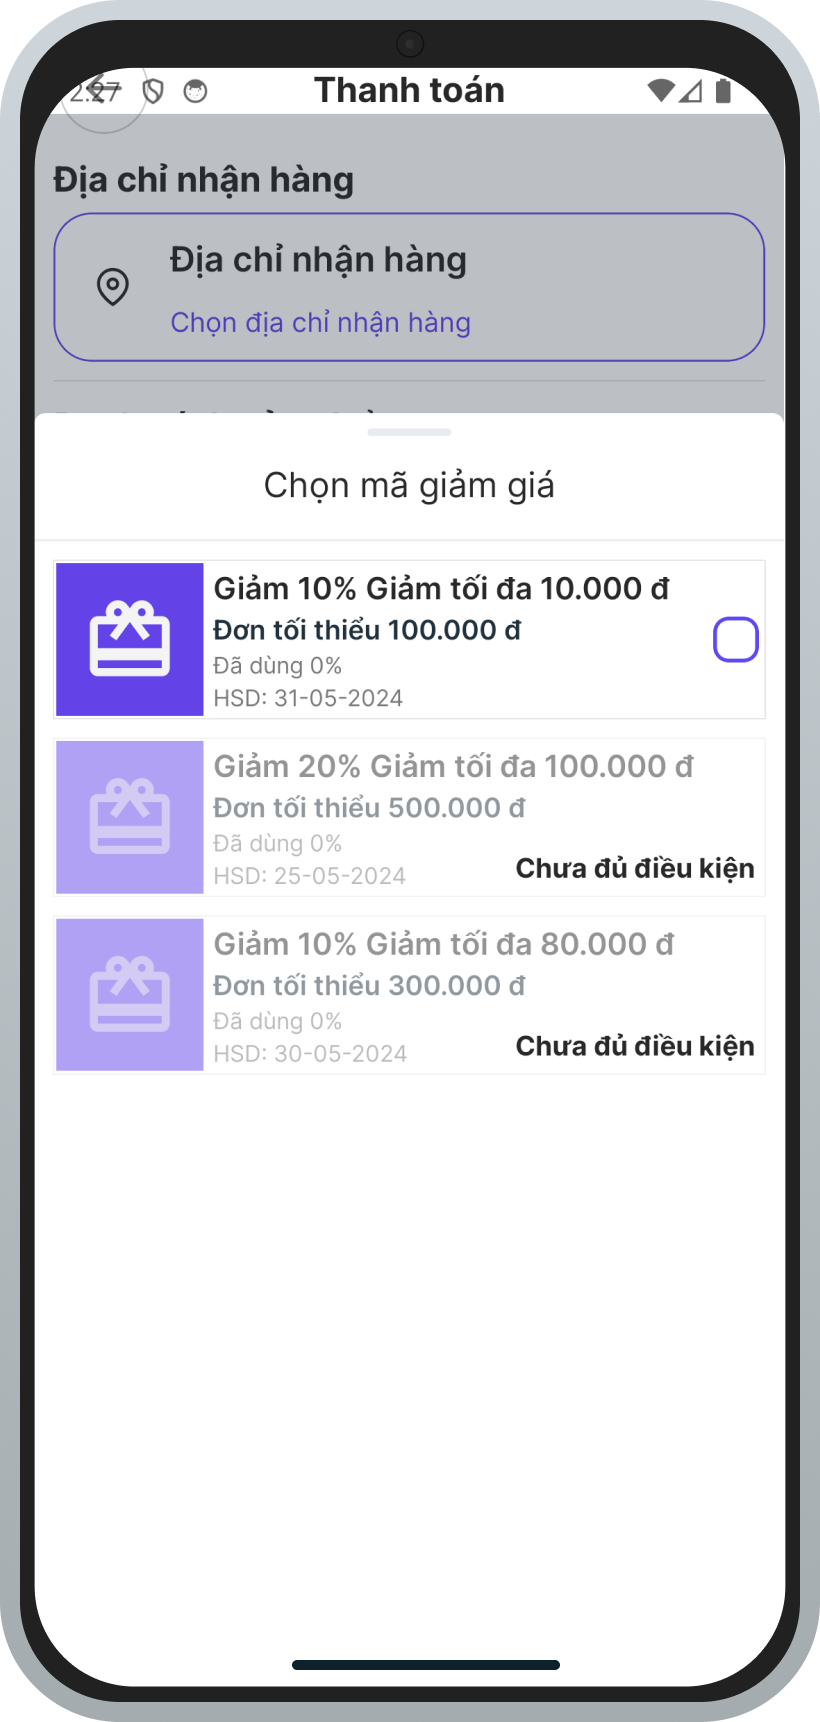
\includegraphics[width=5cm]{Images/Design/User/Main/Mã giảm giá.png}
        \vspace{10pt}
        \centering \caption{Nhập mã giảm giá}
    \end{minipage}
    \end{figure}


      \begin{figure}[H]
    \centering
    \begin{minipage}{0.45\textwidth}
        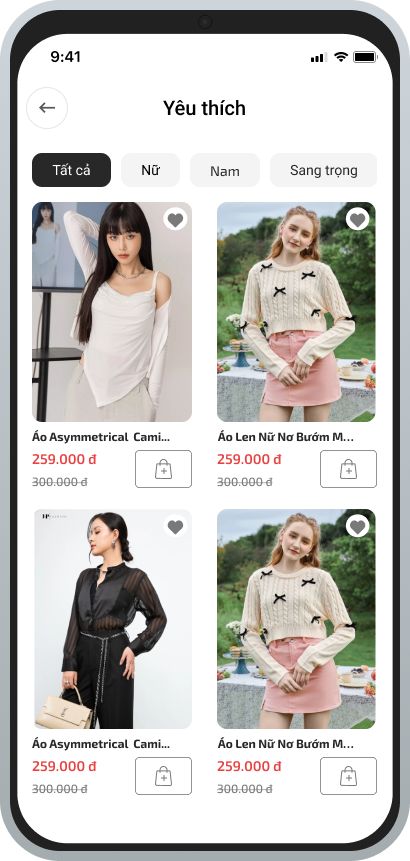
\includegraphics[scale=0.35]{Images/Design/User/Main/Wishlist.png}
        \vspace{10pt}
        \centering \caption{Sản phẩm yêu thích}
    \end{minipage}\hfill
    \begin{minipage}{0.45\textwidth}
        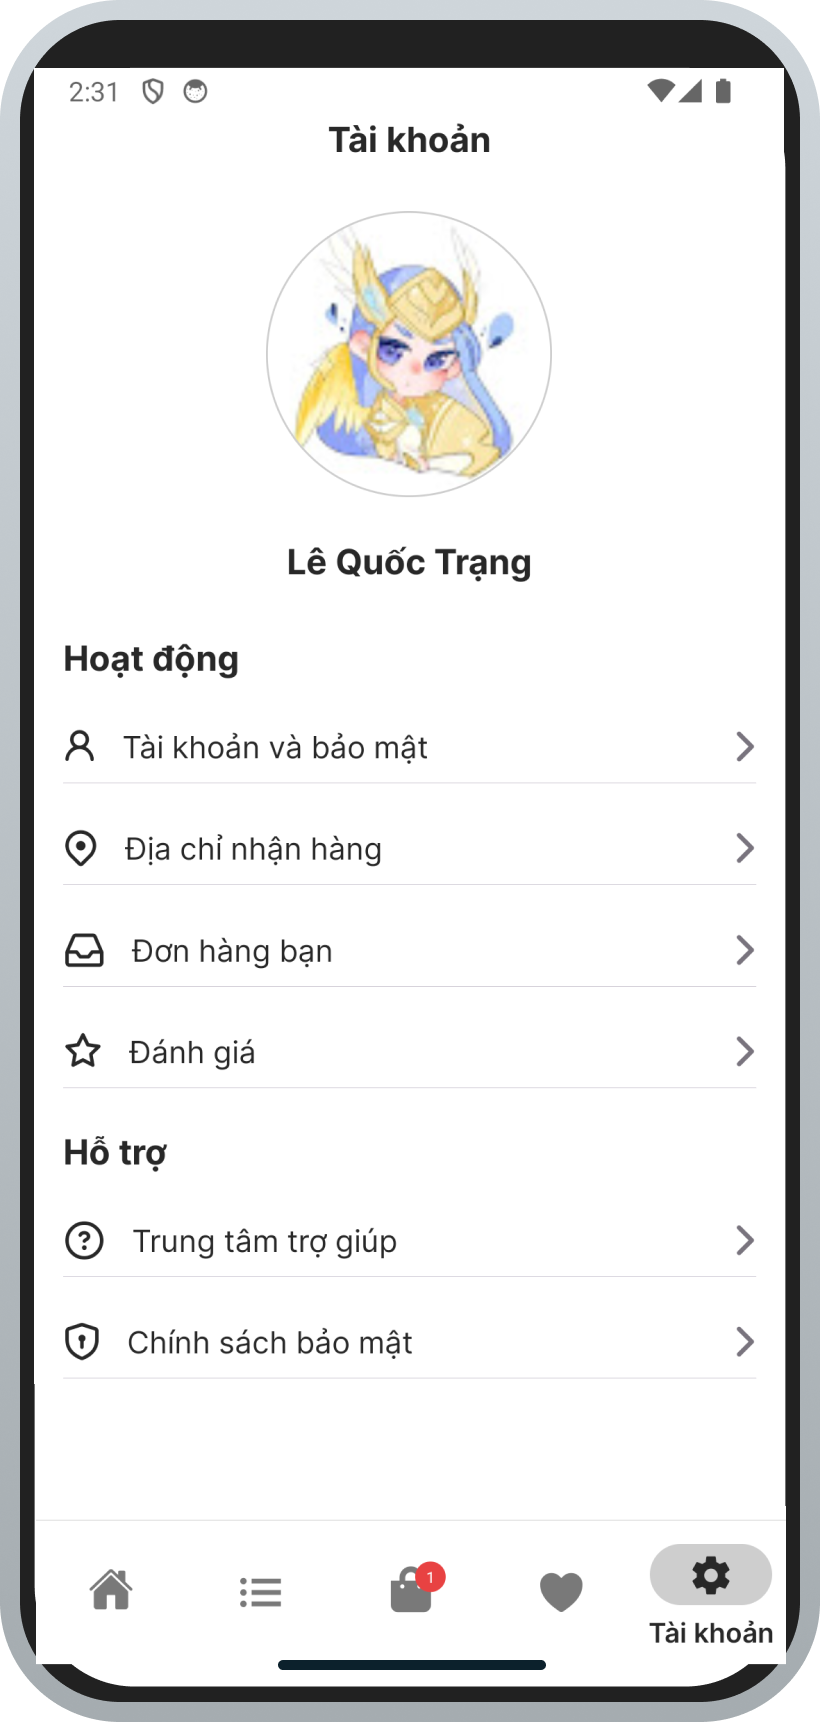
\includegraphics[width=5cm]{Images/Design/User/Main/Profile.png}
        \vspace{10pt}
        \centering \caption{Trang tài khoản}
    \end{minipage}
    \end{figure}

      \begin{figure}[H]
    \centering
    \begin{minipage}{0.45\textwidth}
        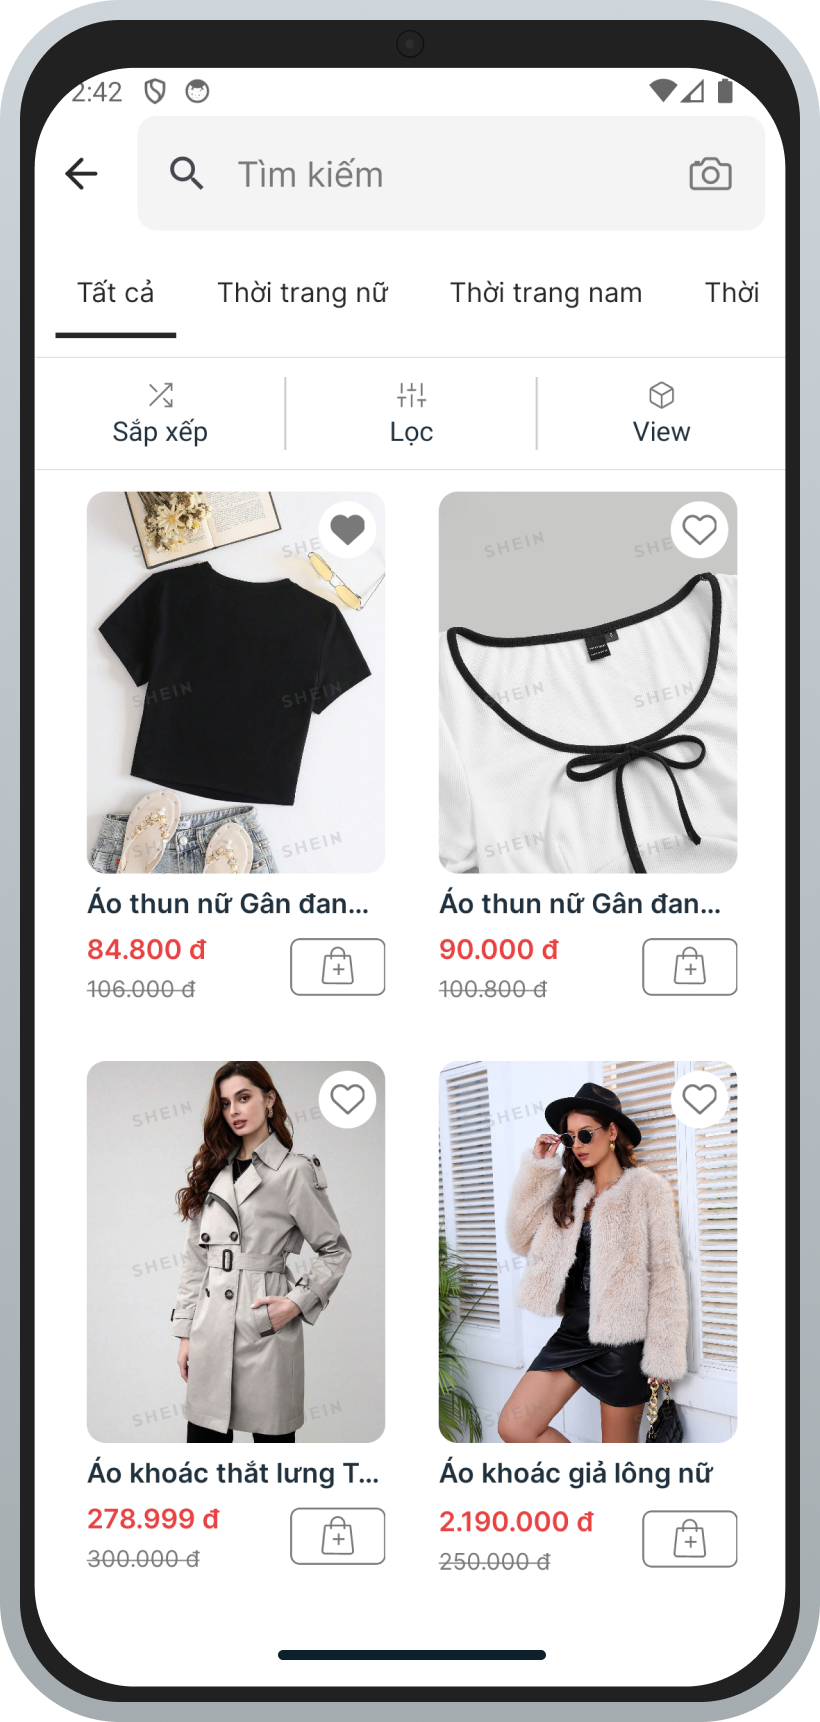
\includegraphics[width=5cm]{Images/Design/User/Main/Filter.png}
        \vspace{10pt}
        \centering \caption{Tìm kiếm, lọc, xem sản phẩm}
    \end{minipage}\hfill
    \begin{minipage}{0.45\textwidth}
        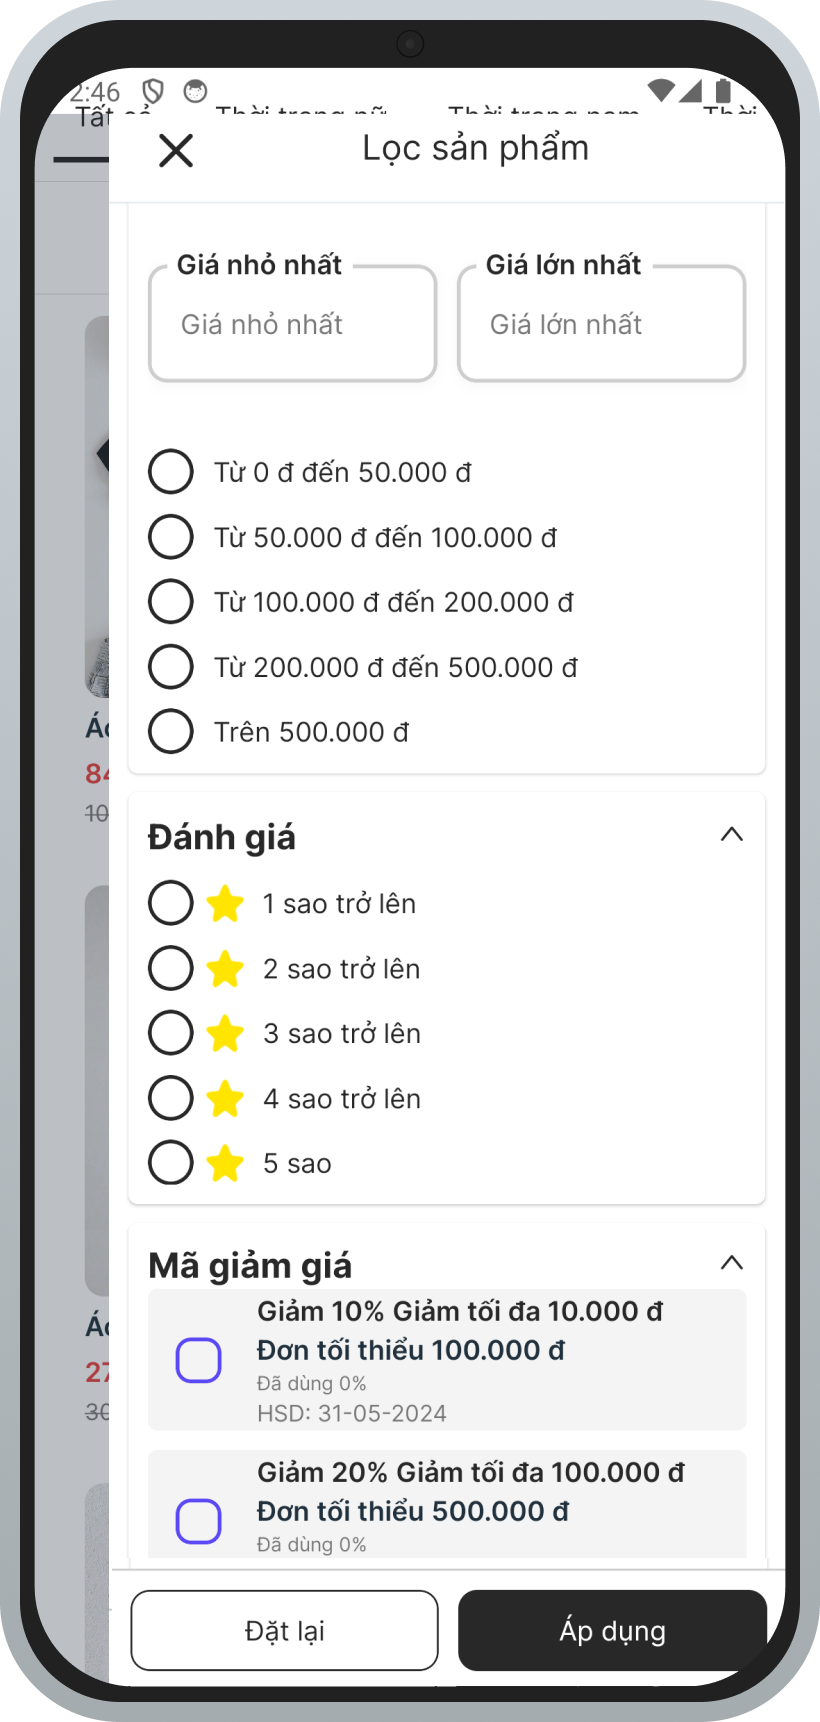
\includegraphics[width=5cm]{Images/Design/User/Main/Filter-1.png}
        \vspace{10pt}
        \centering \caption{Lọc sản phẩm}
    \end{minipage}
    \end{figure}
